
\documentclass[a4paper,twoside,openright,titlepage,
headinclude,,footinclude,BCOR5mm,
numbers=noenddot,cleardoublepage=empty,
tablecaptionabove]{scrreprt}

\usepackage[T1]{fontenc}
\usepackage[utf8]{inputenc}
\usepackage[english]{babel}
\usepackage{amsmath,amssymb}
\usepackage{indentfirst}
%\usepackage[style=philosophy-modern,hyperref]{biblatex}
\usepackage{chngpage}
\usepackage{calc}
\usepackage{listings}
\usepackage{graphicx}
\usepackage{subfig}
\usepackage{lipsum}
\usepackage{shapepar}
\usepackage{pifont}
\usepackage[eulerchapternumbers,subfig,beramono,eulermath,pdfspacing,listings]{classicthesis}
\usepackage{arsclassica}
\usepackage[style=mla,maxnames=3,hyperref]{biblatex}
\input{arsclassica-settings}

\usepackage{microtype}
\usepackage{bm}
\usepackage{listings}
\usepackage{url}
\usepackage{tikz}
\usetikzlibrary{shapes,arrows}
\usepackage{booktabs}
\usepackage{pdfpages} 

\usepackage[dvipsnames]{xcolor}

\usepackage{verbatim}

%opening
\title{Simulated instrumental constraints on brown dwarf atmospheric retrievals for JWST's MIRI.}
\author{Evert Nasedkin}

\begin{document}
	\pagenumbering{roman}
	\pagestyle{plain}
	% !TEX TS-program = pdflatex
% !TEX root = ../ArsClassica.tex

%*******************************************************
% Titlepage
%*******************************************************
\begin{titlepage}
\pdfbookmark{Titlepage}{Titlepage}
\begin{adjustwidth}{-4em}{-4em}
\changetext{}{}{}{((\paperwidth  - \textwidth) / 2) - \oddsidemargin - \hoffset - 1in}{}
    \begin{center}
        {\huge  

        \hfill

        \vfill

        {\spacedlowsmallcaps{\myName}} \\ \bigskip

        {\color{Blue}\spacedallcaps{\myTitle}} 

        }
    	\bigskip
    	\bigskip
		\mySubTitle

        \vfill

        %\includegraphics[width=0.7\textwidth]{TFZSuperEllisse} \\ \bigskip

		
		\medskip
		\textit{Supervised by:}\\ Sascha Quanz \& Polychronis Patapis
        \vfill                      

    \end{center} 
\end{adjustwidth}      
\end{titlepage} 
	% !TEX TS-program = pdflatex
% !TEX root = ../ArsClassica.tex

%*******************************************************
% Titleback
%*******************************************************
\thispagestyle{empty}
\pdfbookmark{Titleback}{Titleback}

\hfill

\vspace{\stretch{2}}

\begin{center}
Evert Nasedkin \\
\smallskip
\textit{Simulated Instrumental Constraints on Sub-Stellar Atmospheric Retrievals for the James Webb Space Telescope's Mid-Infrared Imager.}\\
\smallskip
%Copyright\,\textcopyright\ 2008-2017
\end{center}
\vspace{\stretch{1}}

\medskip

\noindent\textsf{\spacedlowsmallcaps{Titleback}} \\
\noindent
This document was written with \LaTeX{} on Ubuntu using \arsclassica, a reworking of the \classicthesis{} style designed by Andr\'e Miede, inspired to the masterpiece \emph{The Elements of Typographic Style} by Robert Bringhurst. 

\bigskip

\noindent
\textsf{\spacedlowsmallcaps{Contacts}}

\noindent
{\raisebox{-0.33ex}{\ding{43}}}\,\mail{evertn@student.ethz.ch}
	\includepdf{declaration-originality}
	\cleardoublepage
	% !TEX TS-program = pdflatex
% !TEX root = ../ArsClassica.tex

%*******************************************************
% Acknowledgements
%*******************************************************
\pdfbookmark{Acknowledgements}{Acknowledgements}

\chapter*{Acknowledgements}

\begin{flushright}
\itshape
\medskip
--- 
\end{flushright}

\bigskip
\bigskip

	\pagestyle{scrheadings} 
	\pdfbookmark{Abstract}{Abstract}

\chapter*{Abstract}
Following its launch in 2021, the James Webb Telescope will provide the best infrared observations of exoplanets and brown dwarfs to date.
In particular, the Mid-Infrared Instrument (MIRI), will allow for medium resolution spectroscopy across a wide wavelength band, from 4.9-28.8$\mu$m.
This will allow us to derive atmospheric properties of objects at lower temperatures than currently possible. 
MIRI's medium resolution spectrometer (MRS) is an integrated field unit that will perform these observations, providing both spatial and spectral information about targets.
Understanding the instrumental effects is critical to analyzing data from MIRI.
With that in mind, the MIRISIM instrumental simulator was developed to provide observational simulations of the various sub instruments of MIRI.

This thesis improves the implementation of a thin-film fringing model for point sources to MIRISIM, considering how the fringing effect from the detector layers varies with position. 
Fringing is a periodic, wavelength dependent effect, and thus has a strong impact on any spectroscopic observations.
A comparison to the existing model was made, demonstrating the necessity of considering this effect when analyzing data. 
We will improve the fringing removal by identifying the point source location from the constructed data cube, and select the correct fringe flat for removal.

Understanding the instrumental effects is key to quantifying the ability of MIRI to derive atmospheric properties.
Existing literature has considered the NIRCAM instrument and the MIRI Low-Resolution Spectrometer, but to date no retrieval studies have been performed using MIRISIM, or for the MIRI MRS, though it is critical to extend wavelength coverage to improve the results of an atmospheric retrieval.
Model atmospheres will be generated using PetitRadTrans, and processed using MIRISIM and the JWST pipeline to produce a mock observation.
An atmospheric retrieval will be performed, demonstrating to what extent MIRI will be able to retrieve atmospheric parameters such as temperature, pressure and composition. The posterior distributions of these parameters are compared with and without the fringing removal, again demonstrating the importance of correcting for this effect.
	\input{FrontBackMatter/Contents}
	\cleardoublepage
	\pagenumbering{arabic}
	% !TEX TS-program = pdflatex
% !TEX root = ../ArsClassica.tex
\newcommand{\bpic}{$\beta$ Pic b }
\newcommand{\mj}{M$_{j}$}
%************************************************
\chapter{Introduction}
%Meyor queloz
Since the first detection of a planet around a sun-like star \parencite{Mayor1995} the field of exoplanets has evolved rapidly.
Thousands of companions have been identified using the radial velocity and transit detection methods, and a handful have been imaged directly using both ground and space based observatories.
In the last decade, many advances have been made that allow us to begin to characterize the properties of a few of these planets using spectroscopy.
With the launch of the James Webb Space Telescope (JWST) in 2021, and the dawn of the era of extremely large telescopes, we will be able to peer deeper into these planets and further constrain atmospheric or geological properties, allowing us to answer questions about their formation history, climate, and even the prospects for habitability and life.

JWST will operate in near to mid infrared wavelengths, which will provide a new window into studying the atmospheres of exoplanets and brown dwarfs. 
The Mid Infrared Instrument (MIRI) will provide unprecedented spectral resolution in the mid infrared, allowing for the measurement of composition, pressure and temperature. 
Novel instrumentation does not come without challenges. 
Optical and instrumental effects will constrain the ability to which we can measure spectral features, which will ultimately limit the science that can be accomplished.

In this thesis, we will measure the impact of thin-film fringing in the layers of the detectors in the MIRI Medium-Resolution Spectrometer on measurements of atmospheric parameters of brown dwarfs and exoplanets.
This will provide a baseline for determining the level of correction necessary to minimize the impact of fringing, as well as providing a first look into the ability of the MRS to characterize atmospheres.

\section{Exoplanets}
The last quarter century of observations has revealed the diversity of exoplanets and extra-solar systems.
Both the architecture and individual planetary characteristics vary greatly when compared to each other, as well as to our own solar system.
From the hot Jupiters initially found by Mayor and Queloz \parencite{Mayor1995} to the thousands of planets discovered by the Kepler mission, the variety in exoplanets has raised questions about their formation and development, as well as their present day structure, climate, and even prospects for life.
Improvements to observational techniques have allowed us to improve our understanding of these planets.
Secondary eclipse and transmission spectroscopy has opened the door to the study of planets in close orbits to their host stars, while emission spectroscopy of young planet has allowed for constraints on models of planet formation.
Over the next decades, new instruments will be developed that improve sensitivity, allowing us to study smaller, colder and fainter planets: with the ultimate goal of studying atmospheric and surface features of an earth-like planet.

Of particular interest are observable features that allow us to measure physical properties of exoplanets.
The radial velocity (RV) method provides a measure of the planet mass, while a transit can constrain the radius.
Already these properties tell us something about the overall structure of the planet.
Spectroscopy can provide insight into the composition of the planet's atmosphere, as well as its temperature and pressure.
These properties are linked to its age and location of formation in the circumstellar disk.
The atmosphere, combined with the distance between the planet and its star determine the climate of the planet.

%Exoplanet Science Strategy Text: state of field, goals, timelines, summary of methods, biosignatures, formation, tracers, methods, parameters of interest.
% Kepler, Tess, Cheops, RV
\subsubsection{Direct Imaging}
While the majority of exoplanet detections have been made using the radial velocity or transit techniques, direct imaging opens up the possibility of collecting light from the planet itself.
This provides a window into the planet's atmosphere and surface.
Most direct imaging to date has used near-to-mid infrared wavelengths, where the contrast between the thermal emission from the planet and the star is at a minimum, as in Fig. \ref{fig:solarsystem}.
This has its drawbacks: we are so far only able to image young planets that have retained some of the heat from their formation.
 
\begin{figure}[t]
	\centering
	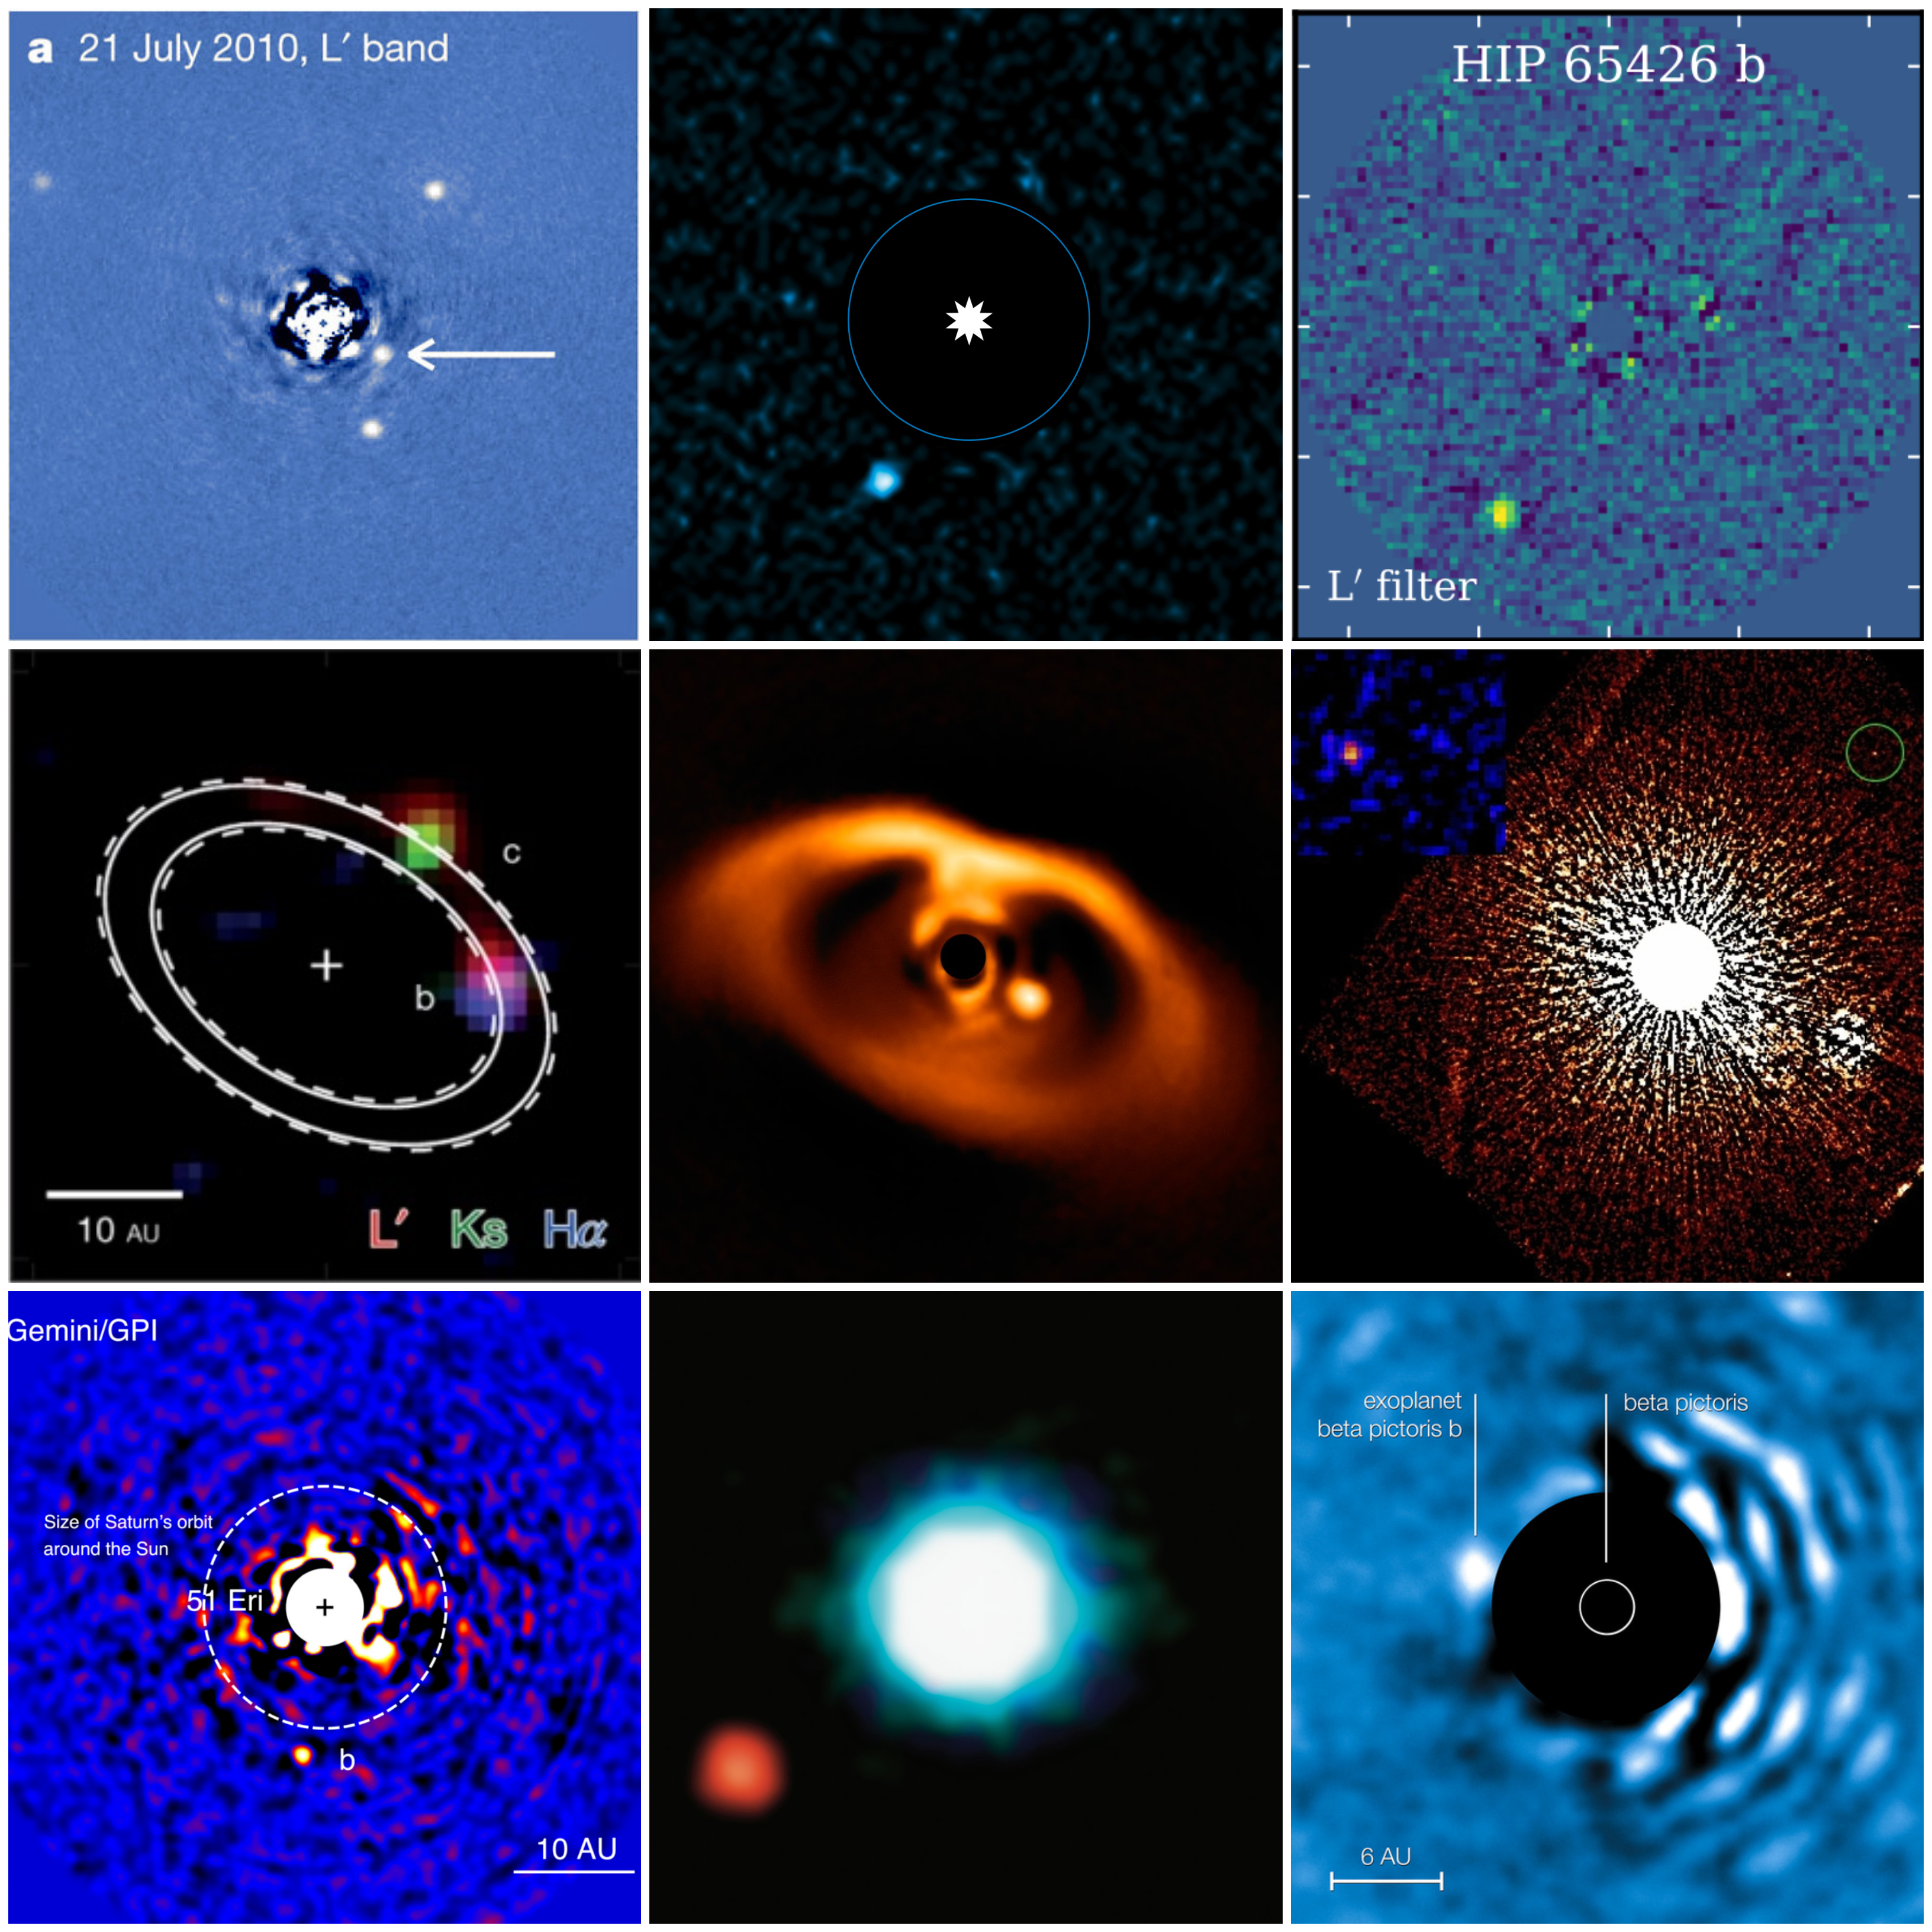
\includegraphics[width=0.75\linewidth]{familyphoto.png}
	\caption{A family portrait of some of the directly imaged exoplanets.
		In order:
	\parencite{Marois2010}, \parencite{Rameau2013}, \parencite{Stolker2020}, \parencite{Sallum2015}, \parencite{Keppler2018}, \parencite{Currie2012}, \parencite{Macintosh2015}, \parencite{Chauvin2004}, \parencite{Quanz2010}.}
	\label{fig:family}
\end{figure}

Direct imaging can make use of both ground and space based observatories. 
However, the high spatial resolution required drives the need for a large primary mirror, limiting the possibilities of space-based telescopes. 
On the other hand, atmospheric turbulence necessitates the use of an adaptive optics equipped facility to observe from the ground. 
Atmospheric absorption due to telluric lines (absorption lines of Earth's atmosphere) also restrict infrared observations to narrow bands.

In addition to the requiring high spatial resolution, it is also challenging to separate the light emitted by the planet from that of the star.
Imaging techniques such as Angular Differential Imaging (ADI) \parencite{Marois2006} and Reference Differential Imaging (RDI) \parencite{Lafreniere2009,Soummer2011} provide methods for reducing the stellar point-spread-function (PSF). %\parencite{Macintosh2006} %ADI
Coronagraphs are optical elements which suppress the stellar PSF through self-destructive interference or physical occultation, depending on the position in the optical path.
The difference in spectra between the planet and the star can also be used to separate the two sources.

\begin{figure}[t]
	\centering
	\includegraphics[width=9cm]{solarsystemcontrast.png}
	\caption{SAO solar system model at 10pc, illustrating the vast difference in luminosity between the Sun and the surrounding planets. However, in the mid infrared the contrast is dramatically reduced at the peak of the planet's emission spectra \parencite{DesMarais2002}.}
	\label{fig:solarsystem}
\end{figure}
Presently, 10m class telescopes such as the Very Large Telescope (VLT) in Paranal, Chile or the Gemini Observatory split between Hawaii and Chile provide the best combination of resolution and instrumentation to perform direct imaging of exoplanets.
The NACO instrument at the VLT provided the first image of an exoplanet in 2004 \parencite{Chauvin2004}.
These observatories are among those equipped with an adaptive optics system, corongraphic instrumentation and near to mid infrared imaging and spectroscopic capabilities to directly image exoplanets, with several exemplar systems becoming standard objects of interest.
While it's terribly interesting to explore the details of each of these objects, we will focus our discussion on objects will be used further in this study, due to their scheduled observation as part of the JWST GTO and Early Release Science (ERS) programs \parencite{Beichman2019}. 
The parameters of these and other directly imaged exoplanets and brown dwarfs are summarized in table \ref{tab:exoplanetparams}. 

In order to understand these objects, we must use a measured spectrum in order to infer physical properties.
Parameters such as the carbon-to-oxygen (C/O) ratio provide insight into formation mechanisms \parencite{Madhusudhan2012}.
A planet that forms near its star will form in a hot region of the circumstellar disk, with a depletion of volatiles due to the high temperature - various species will freeze out at different radii within the disk. 
The measured C/O ratio of a planet will thus depend on its initial formation location and its migration path.
\parencite{Turrini2015} outlines several formation pathways and how the C/O ratio will be affected.
The current climate of exoplanets is also of interest. This requires inferences of atmospheric composition and structure from the spectrum, and will ultimately require time resolved measurements in order to study dynamics and variability. 


 %Not 2019 - summary of JWST science and instruments
 %Exoplanet characterization with JWST MIRI white paper
\subsubsection{VHS-1256 b}
Originally discovered in 2015 \parencite{Gauza2015} as part of the VISTA Hemisphere Survey, VHS-1256b is a late-L dwarf in a 102 AU orbit around an M dwarf.
\parencite{Gauza2015} present astrometric, photometric and spectroscopic data on the planet, finding an age of 150-300 Myr from a moving group association, a luminosity log($L_{bol}/L_{\odot}$) of -5.05$\pm0.22$ and infer a mass of 11.2$^{+9.2}_{-1.8}$ M$_{J}$. 
The effective temperature is found to be 880$^{+140}_{-110}$ K from evolutionary models. 
This is substantially colder than field dwarfs of a similar spectral type (typically 1400K), and so it is proposed that a thick Fe and Mg-Si cloud layer acts to reduce the effective temperature.
Similar findings are presented by \parencite{Rich2016} using Subaru/IRCS.
\begin{wrapfigure}{r}{5.5cm}
	\centering
	\includegraphics[width=5.2cm]{vhs1256b.jpg}
	\caption{VHS-1256b as observed with Subaru/IRCS in the L'-band \parencite{Rich2016}, reduced using the LOCI algorithm \parencite{Galicher2011}.}
\end{wrapfigure}

In \parencite{Miles2018}, methane is detected using KECK/NIRSPEC in the L-band. 
The shallow depth of the feature indicates chemical disequilibrium in the photosphere, as the derived abundance departs from an equilibrium abundance by a factor of 10-100.
However, the best fit model retrieves substantially different parameters for temperature (1240 K) when compared to previously published results.

The wide separation (8") and proximity to Earth make VHS-1256b an ideal target for studying atmospheric properties.
It will be observed as part of the JWST ERS Program \parencite{Hinkley2019}, where a medium resolution spectrum (R$\geq$1700) will be measured from 0.6-28 micron. 
This will enable a more precise measurement of the abundance of methane and other species in the atmosphere, and will allow for investigation of the cloud properties in the mid infrared.
\subsubsection{2M1207b}
Using VLT/NACO, \parencite{Chauvin2004} discovered a low mass companion to the brown dwarf 2MASSWJ 1207334-393254 (2M1207) at a separation of 0.8", or 55AU, shown bottom-center in Fig \ref{fig:family}. 
From their H,K and L'-band photometric observations and NIR spectroscopic measurements, 2M1207b was found to have a spectral type of L5-L9.5, a mass of 5$\pm2$ M$_{J}$ and an effective temperature of 1250$\pm$200K. Followup VLT/NACO observations from \parencite{Mohanty2007} found a higher effective temperature of 1600$\pm$100 K, and a higher mass of 8$\pm$2 M$_{J}$, pushing it closer to the deuterium burning limit. More recent observations have measured periodic signals due to rotation and variability, but failed to constrain the rotation rate due to pointing variance \parencite{Zhou2019}. 

\parencite{Zhou2019} Also present simulated JWST/NIRCam observations of 2M1207b. Access to medium resolution spectroscopy in the mid infrared will allow the characterization of cloud condensate properties. 
The improvement in photometric precision by an order of magnitude will allow better measurement of the rotation rate and variability, and the increase in sensitivity will place lower limits on the possibility of further companions within the system.
It will be observed as part of the JWST GTO program \parencite{Birkmann2019}.

\begin{landscape}
	\begin{table}[t]
		\centering
		\begin{small}
			\begin{tabular}{lllllllll}
				\toprule
				%Name, Mass, Luminosity, Age, Separation, Sep AU, Pri Mass
				\textbf{Name} & \textbf{d [pc]} & \textbf{Mass [M$_{J}$]} & \textbf{Sep [au]} & \textbf{Sep ["]} & \textbf{Age [Myr]} & \textbf{log(L$_{bol}$/L$_{\odot}$)} & \textbf{T$_{eff}$ [K]} & \textbf{References}\\
				\midrule
				\multicolumn{9}{c}{\textbf{Widely separated companions}}\\
				\midrule
				VHS 1256b & $12.7\pm1.0$  & $2\pm1$     & $102$ & $8.1$ & $10^{3}-10^{4}$ & $-5.05\pm0.22$ & $880$ & \parencite{Gauza2015}\\
				Fomalhaut b & $7.704\pm0.028$ & $\leq 2$ & $119$ & $13$ & $440\pm40$ & \ldots & $1600\pm100$ &\\
				\midrule
				\multicolumn{9}{c}{\textbf{Close in companions}}\\
				\midrule
				2M1207b   & $152.4\pm1.1$ & $2\pm1$     & $41$ & $0.8$ & $10\pm3$ & $-4.68\pm0.05$ & $1600\pm100$ &\\
				51 Eridani b & $29.4\pm0.3$ & $2\pm1$   & $13$ & $0.45$ & $23\pm3$ & $-5.06\pm0.2$ & $700$ &  \parencite{Macintosh2015}\\
				\bpic     & $19.3\pm0.2$  & $2\pm1$     & $9$ & $0.4$ & $23\pm3$ & $-3.78\pm0.03$ & $1600\pm100$ & \parencite{Quanz2010}\\
				GJ 504b   & $17.56\pm0.08$  & $3-30$    & $44$ & $2.5$ & $100-6500$ & $-6.13\pm0.03$ & $544$ & \parencite{Skemer2016}\\
				HD 95086b & $90.4\pm3.3$  & $5\pm2$     & $56$ & $0.6$ & $17\pm4$ & $-4.96\pm0.10$ & $1050$  &\parencite{DeRosa2016}\\	
				HR8799b   & $39.4\pm1.0$  & $5\pm1$     & $68$ & $1.7$ & $40\pm5$ & $-5.1\pm0.1$ & $870^{+30}_{-70}$ & \parencite{Marois2008,Skemer2012}\\
				HR8799c   & $39.4\pm1.0$  & $7\pm2$     & $38$ & $0.95$ & $40\pm5$ & $-4.7\pm0.1$ & $1090^{+10}_{-90}$ &\parencite{Marois2008,Skemer2012}\\
				HR8799d   & $39.4\pm1.0$  & $7\pm2$     & $24$ & $0.62$ & $40\pm5$ & $-4.7\pm0.2$ & $1090^{+10}_{-90}$ &\parencite{Marois2008,Skemer2012}\\
				HR8799e   & $39.4\pm1.0$  & $7\pm2$     & $14$ & $0.38$ & $40\pm5$ & $-4.7\pm0.2$ & $1000$ &\parencite{Marois2008,Skemer2012}\\	
				LkCa 15b  & $145\pm15$    & $6\pm4$     & $20$ & $0.08$ & $2\pm1$ & \ldots & \ldots &\\
				PDS 70b   & $113.43\pm0.52$ & $7\pm2$   & $23$ & $0.19$ & $5\pm1$ & \ldots & $900$ &\parencite{Haffert2019}\\
				PDS 70c   & $113.43\pm0.52$ & $4.4\pm1$ & $30$ & $0.24$ & $5\pm1$ & \ldots &  $10^{4}$ & \parencite{Haffert2019}\\
				\midrule
				\multicolumn{9}{c}{\textbf{Nearby Brown Dwarfs}}\\
				\midrule
				WISE 0855   & $2.2\pm0.2$ & $3-10$ & \ldots & \ldots & $10^{3}-10^{4}$ & $-10.5$ &  $225-260$ & \parencite{Luhman2014,Tinney2014}\\
				Luhman 16B   & $1.998\pm0.0004$ & $28.6\pm0.3$ & \ldots & \ldots & $600-800$ & $-4.68$&  $1201$ & \parencite{Sahlmann2015,Garcia2017}\\
				\bottomrule
			\end{tabular}
		\end{small}
		\caption{Summary of directly imaged planet and brown dwarf parameters based on \parencite{Bowler2016} and references therein. Luminosity for WISE 0855 is calculated in H band.}
		\label{tab:exoplanetparams}
	\end{table}
\end{landscape}
\section{Brown Dwarfs}
Brown dwarfs are the low mass result of a failed star formation process.
On the low end of the mass scale, an object is considered a brown dwarf at >13M$_{J}$, which is the deuterium burning limit.
By 75M$_{J}$, the object is heavy enough to sustain hydrogen fusion and the object is considered a star.
However, there have recently been observations even lower mass brown dwarfs, down to several Jupiter masses, raising questions of formation processes \parencite{Luhman2014}.
It is generally thought that brown dwarfs form during the gravitational collapse of a molecular cloud, while exoplanets form through a core accretion process in a circumstellar disk.
Observations of high mass companions and low mass field objects then challenge these standard models.

While brown dwarfs are objects of scientific interest in their own right, we are particularly interested in their use as analogs for exoplanets due to their similar temperatures and pressures.
Without the issue of contrast between an exoplanet and its host star, brown dwarfs are ideal targets for medium and high resolution spectroscopic characterization.
As shown in table \ref{tab:exoplanetparams}, they are also some of the closest known objects to the solar system, with several having been observed at around 2pc.

\subsection{Observational Properties}
Brown dwarfs are characterized by their spectral type, either by comparison to spectral templates, using indicies derived from spectral parameters or through broadband photometric comparison \parencite{Helling2014}.
Directly imaged exoplanets can also be classified using brown dwarf spectral types.
Unlike stars which maintain their temperature and luminosity through fusion, brown dwarfs cool and change their spectral type with age, leading to a degeneracy between mass and age \parencite{Burrows2001}.
This spectral series is shown in Fig. \ref{fig:bdspec}.

As a brown dwarf cools and contracts over time, its surface gravity will increase, leading to the use of log(g) as a tracer of age \parencite{Manjavacas2014}.
Young, low surface gravity objects are particularly comparable to directly imaged exoplanets.
In these young objects, clouds are a nearly universal feature \parencite{Cooper2003,Helling2014}, with thicker cloud decks appearing in low gravity objects \parencite{Helling2014}.

\begin{figure}[t]
	\includegraphics[width=\linewidth]{bdspectral.png}
	\caption[Brown Dwarf Spectra]{Near Infrared spectral series of brown dwarfs from early-M to early-Y as shown in \parencite{Helling2014}.}
	\label{fig:bdspec}
\end{figure}

\subsubsection{L-Type}
L-dwarfs are the hottest brown dwarfs, with typical effective temperatures between 1300K and 2100K \parencite{Burrows2001}.
L-type spectra are notable for the disappearance of VO and TiO NIR absorption lines and the onset of molecular absorption features such as H$_{2}$O and CO, with CH$_{4}$ appearing in late L types \parencite{Manjavacas2014}.
Further key features of L-dwarfs is the formation of iron and silicate condensate, as well as the growth of neutral alkali lines \parencite{Burrows2001}.
\subsubsection{T-Type}
As a brown dwarf ages it moves towards a T-type spectrum. 
The L/T transition occurs  with the appearance of both CH$_{4}$ and CO absorption, and is characterized by increasingly blue J-H colour as the temperature decreases.
There are several proposed mechanisms for this transition, with cloud fragmentation due to particle microphysics \parencite{Burningham2017} and convection processes being two examples \parencite{Tremblin2015}.
Both T- and L-dwarfs are highly variable due to complex atmospheric dynamics ranging from clouds to banding structures to hot spots and more \parencite{Biller2017}.
\parencite{Vos2019} presents how monitoring with JWST/MIRI will be able to constrain the mechanism behind this transition.
\subsubsection{Y-Type}
Y-type dwarfs are ultracool objects first discovered in \parencite{Cushing2011}. 
With such cold temperatures, they contain deeper water and methane absorption features than present in T-dwarfs, and likely have ammonia present as well.
Atmospheric models suggest typical temperatures between 300-500 K, which places them as the coldest detected and spectroscopically measured brown dwarfs to date \parencite{Cushing2011}.

\subsubsection{WISE 0855-0714}
WISE-0855 is the coldest known brown dwarf at 250K, with an inferred mass of 5 M$_{J}$ \parencite{Luhman2014}, and a Y2-4 spectral type \parencite{Leggett2015}.
Although faint, with a J-band magnitude of 25, its proximity to the sun makes allows for its spectral characterization.
Present measurements indicate the presence of ammonia \parencite{Leggett2015} and water clouds \parencite{Morley2014,Faherty2018} in its atmosphere.

\begin{wrapfigure}{r}{5.5cm}
	\centering
	\vspace{-1em}
	\includegraphics[width=5.2cm]{wise0855im.jpg}
	\caption{W2, epoch 1 image of WISE0855 on top of a known background clump. The green circle represents the location of WISE0855, the yello is the position of the background source \parencite{Wright2014}. }
	\label{fig:wise0855im}
	\vspace{-6em}
\end{wrapfigure} 
WISE 0855, along with other Y-dwarfs will be the subject of JWST investigation \parencite{Oliveira2015,Oliveira2019}.
Its low mass and cold temperature make it the closest analog to solar system objects, especially to Jupiter. 
Further observations will allow for tighter constraints on atmospheric composition and cloud properties, as well as insight into whether such objects are the result of a star-like formation process or are an ejected, free floating planet \parencite{Beichman2014}.
\section{Motivation}
\subsection{Current Status of Atmospheric Characterization}
Both exoplanets and brown dwarfs raise interesting questions with regards to atmospheric properties, but there are substantial challenges both in gathering the data necessary to answer them and modeling the physics underlying the observable parameters. 
The best methods currently in use involve taking spectroscopic data and inferring atmospheric properties from the spectral features.
The light we measure may be thermal emission from the planet, where it is absorbed and scattered as it passes through the planet's atmosphere, or it may be light from the planet's host star which passes through the upper layers of the atmosphere.
These provide complementary information about the composition and structure of the atmosphere, probing different altitudes and pressures.
While a more complete overview of exoplanet atmospheres is covered in the literature, e.g. \parencite{Bozza,Madhusudhan2014,Seager2010}, we will briefly summarize the current methods used and what has been learned so far.
%Transmission spectroscopy, facilities, atmosphere, climate, condensates
 % Exoplanet atmosphere measurements, hr8799 photometry/spec, prospects for jw
 %Exoplanet atmospheres textbook: observation, models, spectroscopy, solar system atmospheres
 %Atmospheric char with MIRI (coron,LRS, not MRS I think)
%\parencite{Madhusudhan2016} %Chemistry, Formation, Habitabiltiy
\subsubsection{Transmission Spectroscopy}
Many exoplanets have been discovered using the transit technique in which the planet passes in front of its host star, blocking a small fraction of its light.
Through time series observations, particularly with satellites such as Hubble, Kepler, and TESS, we can observe this dip in stellar brightness, and infer properties of the planet.
A key feature of this observation is that in the case the planet has an atmosphere, the brightness dip is wavelength dependent.
Depending on the wavelength, different species within the atmosphere will absorb the light to a greater or lesser extent.
Thus if a species is abundant within the atmosphere, it will create deep absorption features, which will make the apparent radius of the planet larger, increasing the transit depth.
Measuring this radius variation is the procedure of transmission spectroscopy, and is used to probe the composition and structure of the upper atmospheres of transiting planets.
In addition to transmission spectroscopy, secondary eclipse spectroscopy is another transit measurement that uses the reflected light and thermal emission of the planet, and measures the dip in total luminosity as the planet passes behind its host star.
This provides a more direct measurement of the planet's reflection or emission spectrum.
\parencite{Kreidberg2018} presents a concise overview of transmission and eclipse spectroscopy.

Transmission spectroscopy attempts to answer questions about atmospheric composition, formation history and present climate.
To date, water features and carbon-bearing molecules have been detected, though molecules commonly present in the solar system such as methane and ammonia have not been detected, largely due to lack of long wavelength coverage and the high temperatures of most transiting planets \parencite{Lee2012,Kreidberg2018}.
The C/O ratio has been measured in some hot Jupiters, including WAST-12b, which provides a trace for formation history and current composition \parencite{Madhusudhan2011}. 
For WASP-12b, the high C/O ratio (>1) and the lack of an observed thermal inversion in the highly irradiated atmosphere both stand in contrast to theoretical predictions, and demonstrate the necessity for improvements in atmospheric and formation modeling \parencite{Madhusudhan2011}.
In other atmospheres, nitrogen chemistry has been observed, and condensates (clouds and hazes) are nearly universal \parencite{MacDonald2017}.

Future observations will increase the spectral resolution of transit observations, and will also extend the wavelength coverage. 
By probing the mid infrared, it may be possible to determine the composition of the clouds observed, and place tighter constraints of the abundances of species present within atmospheres \parencite{Kreidberg2018}.

\subsubsection{Emission Spectroscopy}
In contrast to transit observations, emission spectroscopy is a direct measurement of the light emitted by the planet, usually in the infrared, where the planet's luminosity peaks due to Wein's law.
Due to the low levels of flux emitted from most planets, most emission spectroscopy to date has been low to medium resolution, in order to collect enough light for measurement. 
However, this has already allowed us to begin to answer similar questions as posed for transmission spectroscopy.
What are these atmospheres made of? How did these planets form?
In many ways though, emission and transmission spectroscopy provide complementary information, and multiple ways of approaching these problems. 
Due to the different wavelength regimes, they are able to identify different species and probe different atmospheric depths. 

Only recently has high quality exoplanet emission spectroscopy become possible, and a comprehensive overview is provided in \parencite{Biller2018}.
Measurements of H$\alpha$ emission in LkCa 15b have allowed for inferences of the mass accretion rate of a forming planet \parencite{Sallum2015}, while observations of the PDS 70 system indicate the presence of a circumplanetary disk around PDS 70b \parencite{Keppler2018,Christiaens2019}.
With integrated field spectroscopy, \parencite{Hoeijmakers2018} show how spectroscopy can identify the presence of molecular species in a spectrum and how this can be used to discover companions within the contrast-limited regime.
Using the VLTI/GRAVITY instrument, which combines light from all four Unit Telescopes (UTs) of the VLT into a single interferometer, medium resolution (R=500) spectra have been taken of HR 8799e \parencite{Lacour2019} and \bpic \parencite{GRAVITYCollaboration2019}, the latter of which is shown in Fig. \ref{fig:gravitybpic}. 
These spectra represent some of the best data available to date for exoplanets, and additional observations of well-known directly imaged planets are planned in the near future.
While not yet accomplished for an exoplanet, it may be possible in the near future to longitudinally map cloud features of exoplanets, as has already been accomplished for brown dwarfs using the CRIRES instrument \parencite{Crossfield2014}.
\begin{figure}[t]
	\includegraphics[width=\linewidth]{gravitybpic}
	\caption{Flux calibrated K-Band emission spectrum of \bpic as measured using the VLTI/GRAVITY at R=500 \parencite{GRAVITYCollaboration2019}, along with the GPi K-Band spectrum from \parencite{Chilcote2017}.}
	\label{fig:gravitybpic}
\end{figure}\\

As most older planets will emit primarily in the thermal infrared, JWST/MIRI will provide unprecedented capabilities at imaging and characterizing these systems.
\parencite{Danielski2018} shows that the MIRI LRS will allow for the detection of ammonia in the coldest targets, as well as characterize the abundances of other molecules such as CH$_{4}$, H$_{2}$O, CO$_{2}$ and PH$_{3}$.
Many direct imaging observations of exoplanets have been proposed as part of the JWST GTO and ERS programs. In a white paper, \parencite{Beichman2019} discuss how JWST will provide new insight into exoplanet atmospheres using direct emission imaging and spectroscopy, while \parencite{Line2019} examines the possibility of characterizing terrestrial planets using thermal emission spectroscopy. 

\subsection{JWST Studies}
With the launch of JWST imminent, many proposals have been made to cover a wide range of science cases, as well as performing instrumental testing, calibration and validation.
Exoplanet science is well represented within these first observations, and several of the proposals will be presented here.
\subsubsection{Early Release Science}
The Early Release Science program is an initiative designed to help scientists develop an understanding of the instruments available on JWST, as well as the tools needed to process the data. 
Thus the ERS provides an extensive catalog of public data immediately upon observation, and will take place within the first 5 months of JWST science operations.
Both a transiting program \parencite{Bean2018} and a direct imaging program \parencite{Hinkley2019} have been approved.
The direct imaging proposal has 52 hours observing time in order to take data using the full range of JWST instrumentation and observing modes.
The goal is to image a representative sample of known directly imaged planets, including VHS-1256b, in order to develop the tools and techniques necessary to push the limits of the instrumentation.

\subsubsection{GTO Programs}
In addition to the ERS program, the Guaranteed Time Observations (GTO) program is designed to provide scientists who helped in the development of JWST hardware and software with a set amount of observing time. 
Many GTO programs focused on exoplanet science have been approved, including spectroscopic studies of 2M1207b and other commonly studied systems \parencite{Birkmann2019}.
Brown dwarf science is also well represented within the GTO program, with WISE-0855 receiving full spectroscopic coverage from 0.6-28 $\mu$m \parencite{Oliveira2019}.
Details of the observations for VHS-1256b, 2M1207b and WISE-0855 are discussed in \ref{sec:obs}.

\subsection{Biosignatures and Future Missions}
While JWST will provide higher spectral and spatial resolution in the infrared than any previous observatory, many questions will remain open for future missions.
One of the ultimate unanswered questions in science is "Are we alone?".
The detection of biosignatures in the near future with next generation 40m class telescopes \parencite{Lopez-Morales2019} or proposed space missions such as LIFE \parencite{Quanz2019} and LUVOIR \parencite{Luvoir2019} may provide our best chance at answering such questions.
Instruments such as METIS on the ELT will offer high resolution (R=100000) integral field spectroscopy of nearby terrestrial planets, while both proposed space missions will have the spatial and spectral resolution necessary to characterize a nearby earth like planet.
With such a goal in mind, it is necessary to develop the technical capabilities in both theory and observation order to achieve such ambitious goals in the not-so-distant future.

\section{Thesis Overview}
With sufficient background and motivation, we will now outline the remainder of this thesis.

Chapter 2 will provide a more extensive background of the James Webb Space Telescope, and in particular the MIRI Medium Resolution Spectrometer (MRS).
We will outline the principle optical components dedicated to integral field spectroscopy, as well as the detector characteristics of MIRI.
This will provide the necessary background to understand the instrumental and optical effects discussed in Chapter 3.

The third chapter examines the fringing effect in the MIRI MRS instrument.
We discuss the optical effects that result in fringing patterns, as well as outlining current and future strategies for fringe correction.
We describe the creation and processing of our mock observations using the MIRI instrumental simulator and the JWST data reduction pipeline.
With the degraded spectra from the simulated data, we measure the impact of fringing on spectral extraction using cross correlation techniques, and and how this impacts molecular mapping studies.
This in turn motivates Chapter 4, where the species identified using molecular mapping can justify the inclusion or exclusion of particular species in an atmospheric retrieval.

In Chapter 4 we explore atmospheric retrievals with the MIRI MRS.
We outline our procedure for performing a retrieval using the petitRADTRANS radiative transfer code and Multinest as an implementation of the nested sampling strategy for parameter space exploration
We measure the impact of fringing on parameter estimation, and also investigate how observing parameters will impact retrievals, discussing the advantages and challenges of studying atmospheres in the mid infrared.

Finally we summarize and discuss our findings and future investigations in the final chapter.


	\chapter{MIRI: The Mid-Infrared Instrument}
MIRI is an instrument that will provide unique capabilities for studying exoplanets and other cold and distant objects. This chapter will provide a detailed overview of the technical details and capabilities of the instrument. A complete description of MIRI is provided in a series of papers from \parencite{MIRI1,MIRI2,MIRI3, MIRI4,MIRI5,MIRI6,MIRI7,MIRI8,MIRI9}.
%MIRI is an imaging and spectroscopic instrument on board the James Webb Space Telescope (JWST). 
%
%
\section{The James Webb Space Telescope}
JWST is a 6.5 m space based observatory built in collaboration between NASA, ESA and CSA that will be located in a halo orbit at the L2 Earth-Sun Lagrange point. 
As the successor to the Hubble Space Telescope and the Spitzer Space Telescope, it will provide a new perspective for infrared astronomy. 
It is currently scheduled to launch in March 2021.

James Webb is fully optimized for infrared astronomy. 
To reduce instrumental thermal background, the entire telescope will operate at cryogenic temperatures. 
A large sun-shield will help block solar infrared radiation.
The lightweight beryllium mirrors are coated in gold to maximize reflectivity out to the mid infrared.

Of key interest to exoplanet science is the both the sensitivity and spatial resolution of the instrument. 
With its 6.5 m primary, JWST will have a spatial resolution from 0.01" at 0.6 micron to 0.92" at 29 micron.
The increase in sensitivity is due in part to the larger collecting area, but also to advances in detector technology since the previous generation of infrared observatories.
For example, the MIRI instrument will have a minimum detectable flux of 0.13 $\mu$Jy at 5.6 micron and a 10 000 second integration, or roughly a factor of 1000 better than what was possible with the Spitzer Space Telescope \parencite{MIRI9}.
\begin{figure}[t]
	\includegraphics[width=\linewidth]{assembled.jpg}
	\caption{The James Webb Space Telescope during integration of the telescope into the Spacecraft Element \parencite{assembled}. }
	\label{fig:jwst}
\end{figure}

There are four primary instruments that constitute the Integrated Science Instrument Module (ISIM). 
Near-Infrared Camera (NIRCam), which provides imaging with coronagraphic capabilities from 0.6-5 micron.
The Near-Infrared Spectrograph (NIRSpec) provides fixed slit and integrated field unit spectroscopy capable of analyzing multiple objects simultaneously, and operates in the same wavelength range as NIRCam.
The Fine Guidance Sensor/ Near-Infrared Imager and Slitless Spectrograph (FGS/NIRISS) allows for low and medium resolution spectroscopy with high photometric stability, as well as aperture masking interferometry. 
The final instrument, MIRI, is the subject of this thesis.

\section{MIRI}
The Mid-Infrared Instrument (MIRI) provides imaging, fixed slit and integrated field spectroscopy between 4.8 and 28 micron \parencite{MIRI2}.
These sub-instruments are enclosed in a closed-cycle cooler to maintain a temperature of 6.7 K in order to reduce the thermal background.
At its most sensitive, MIRI is about 1000$\times$ more sensitive than comparable instrumentation on Spitzer. 
Sub-instrument sensitivities are shown in Fig. \ref{fig:sensitivities}.
While this will prove tremendously valuable for exoplanet science, it will also allow exploration of star formation, extra galactic astronomy and high-redshift observations. 
These and further science cases are described in \parencite{MIRI1}. 
In its imaging mode, MIRI can operate with either a Lyot or 4-Quadrant-Phase-Mask coronagraph to reduce stellar glare, the MRS is not equipped with such an element. 
Thus its use for exoplanet observations is restricted to highly separated or bright targets. 
It may also be possible to use the differences between the host star and companion spectra in order to image close in planets.

 %MIRI intro

\begin{table}[t]
	\begin{footnotesize}
	\centering
	\begin{tabular}{l|lll}
		\toprule
		\textbf{Subsystem} & \textbf{$\lambda$ Range [$\mu$m]} & \textbf{Px Scale ["/px]} & $\Delta\lambda/\lambda$\\
		\midrule
		Imaging & 5-28 & 0.11 & 3.5-16.1\\
		4QPM Coronagraphic Imaging & 10.65,11.4,15.5 & 0.11 & 14.1-17.2\\
		Lyot Coronagraphic Imaging & 23 & 0.11 & 4.1\\
		Low Resolution Spectroscopy & 5-12 & 0.11 & 100 @ 7.5$\mu$m\\
		Medium Resolution Spectroscopy & 4.9-28.8 & 0.196-0.273 & 1550-3300 \\
		\bottomrule
	\end{tabular}
	\caption{Summary of MIRI observing modes.}
	\label{tab:mirimodes}
	\end{footnotesize}
\end{table}
\begin{figure}[h]
	\centering
	\includegraphics[width=0.8\linewidth]{mirisensitivities.png}
	\caption{Sensitivities of MIRI sub-instruments for an SNR of 10, with a 10 000s integration \parencite{MIRI1}.}
	\label{fig:sensitivities}
\end{figure}
\section{The Medium Resolution Spectrograph}\label{sec:mrs}
The Medium Resolution Spectrograph (MRS) consists of four integrated field spectrographs projected onto two detectors, covering 4.8-28 micron with a spectral resolution varying from R=1700 to R=3500.
Its FoV ranges from 4"$\times$4" to 7.7"$\times$7.7".
While a full description of the MRS is given in \parencite{MIRI6}, in this section we will outline the optical design of the instrument.
\begin{table}[t]
	\begin{small}
	\centering
	\begin{tabular}{l|lc|cccc}
		\toprule
		\textbf{Channel} & \textbf{Sub-band} & \textbf{Band} & \textbf{Detector} & $\lambda$ \textbf{Range [$\mu$m]} & \textbf{FoV [as]} & $\lambda$/$\Delta\lambda$\\
		\midrule
		\multirow{3}{*}{1}  &Short & 1A & \multirow{3}{*}{SW}   & 4.83 - 5.82 & 3.46$\times$3.72 & 3500 \\
							&Medium & 1B &						& 5.62 - 6.73 & 3.46$\times$3.72 & 3500 \\
							& Long & 1C&						& 6.46 - 7.76 & 3.41$\times$3.72 & 3300 \\
		\midrule
		\multirow{3}{*}{2}  &Short & 2A & \multirow{3}{*}{SW}   & 7.44 - 8.90 & 4.16$\times$4.76 & 3000 \\
							&Medium & 2B &						& 8.61 - 10.28 & 4.16$\times$4.76 & 3000 \\
							& Long & 2C&						& 9.94 - 11.87 & 4.12$\times$4.76 & 3000 \\
		\midrule
		\multirow{3}{*}{3}  &Short & 3A & \multirow{3}{*}{LW}   & 11.47 - 13.67 & 6.00$\times$6.24 & 2700 \\
							&Medium & 3B &						& 13.25 - 15.80 & 5.96$\times$6.24 & 2300 \\
							& Long & 3C&						& 15.30 - 18.24 & 5.91$\times$6.24 & 2300 \\		
		\midrule
		\multirow{3}{*}{4}  &Short & 3A & \multirow{3}{*}{LW}   & 17.54 - 21.10 & 7.14$\times$7.87 & 1700 \\
							&Medium & 3B &						& 20.44 - 24.72 & 7.06$\times$7.06 & 1700 \\
							& Long & 3C&						& 23.84 - 28.82 & 6.99$\times$7.87 & 1500 \\			
		\bottomrule
	\end{tabular}
	\end{small}
	\caption{Properties of the MIRI MRS channels \parencite{MIRI6}.}
	\label{tab:mrs}
\end{table}

\subsection{Coordinates}
There are three primary coordinate systems in use with JWST/MIRI-MRS, of which two will be relevant for this thesis, with the detector and local MRS coordinates described in Fig. \ref{fig:mrscoords} \parencite{Argyriou2020}.

The detector coordinate grid is formed by counting x/y pixels, as well as the slice number.
Each of the two MRS detectors is an array of 1032$\times$1024 pixels, though only 1024 are photosensitive in the horizontal direction.
Each image slice from the IFU appears as a curved stripe on the detector, though neighboring stripes on the detector do not correspond to neighbouring slices of the image. 

The local MRS coordinate system is described in terms of $\alpha,\beta$ and $\lambda$. The continuous $\alpha$ coordinate is the along slice direction, while $\beta$ is perpendicular and discrete, corresponding to the slice number. $\lambda$ is the wavelength. Both $\alpha$ and $\lambda$ are fit by a second order polynomial to account for along and across slice distortion \parencite{MIRI6}. Each detector sub array has its own mapping to $\alpha,\beta,\lambda$ space, due to the differences in FoV, slice count, distortion and spectral resolution.

The third coordinate frame is the global coordinate system of JWST itself, V1,V2,V3. The V1 coordinate refers to the symmetry axis of the telescope, V3 points towards the foldable secondary mirror support structure strut. V2 completes the coordinate system, being orthogonal to V1 and V3. This coordinate system will not be used in this thesis.

\begin{figure}[t]
	\includegraphics[width=\linewidth]{coordinates.png}
	\caption{Description of the MRS detector (x,y,s) coordinate system to the local MRS ($\alpha,\beta,\lambda$) cube coordinates. \textbf{Top}: Detector coordinates. Note that the consecutive stripe numbers s$_{i}$, s$_{i+1}$ correspond to neighbouring image slices. \textbf{Bottom}: Description of the (invertible) detector-to-cube transformation \parencite{Argyriou2020}.}
	\label{fig:mrscoords}	
\end{figure}

\begin{figure}[t]
	%\includegraphics[width = 0.45\linewidth]{}
	%\includegraphics[width = 0.45\linewidth]{}
	\caption{Detector images of a spatially and spectrally flat calibration source for the SW detector (left) and LW detector (right).}
	\label{fig:flatfield}
\end{figure}
\subsection{Integral Field Spectroscopy}
As an integrated field spectrograph (IFS) consisting of 4 integrated field units (IFUs), the MRS provides both spatial and spectral information.
This is accomplished by slicing the on sky image, and performing spectroscopy on each of the image slices. 
Here we will step step through some of the key optical systems used to accomplish this, while a more detailed description of the optics is given in section 2 of \parencite{MIRI6}.

A series of optics picks off a FoV from the telescope beam, and directs it to the IFU slicing mirrors, where the focal plane is re-imaged. 
The image slicer consists of an array of thin mirrors at unique angles, in order to separate different spatial slices of the on-sky image.
The across slice width is equal to the FWHM of the Airy pattern at the shortest wavelength of the given IFU.
There are a total of 4 image slicers, one for each of the MRS channels.
Each slice is then collimated, and directed to a diffraction grating. Each channel has 3 separate gratings, each covering approximately a third of the wavelength range of each channel. 
Thus it requires 3 total exposures to cover the wavelength range of a channel.
Channels one and two are each projected onto separate halves of a single detector, as are channels 3 and 4.
As such, multiple wavelength ranges are imaged simultaneously, and it requires only 3 exposures in order to cover the entire MRS wavelength range. 
\subsection{Detectors}
MIRI uses three arsenic-doped silicon (Si:As) impurity band conduction (IBC) detectors descended from those used in the Spitzer Space Telescope.
Each detector uses a 1024$\times$1024 pixel format.
One detector is used for the imaging and LRS modes, while the remaining two detectors are used in the MRS.
The full technical details of the detectors are described in \parencite{MIRI7}.

Si:As IBC detectors are ideal for mid-infrared measurements.
Each detector is built onto a high resistivity transparent contact. 
A 25-35 micron thick, heavily arsenic doped layer acts as the absorption layer, with an electric field maintained across the layer in order to transport the generated photoelectron.
A transparent contact layer provides a connection to the detector electronics, where the signal is amplified and read out.
A schematic of the layers in the detector is provided in the context of the fringing effect in Fig. \ref{fig:layers}.
These detectors have a quantum efficiency that is wavelength dependent, and provides a fundamental limitation on the sensitivity.
Precise measurement of this photon-to-electron conversion efficiency is critical for photometrically calibrating observations. 
The efficiencies are shown for each sub-band of the MRS detectors in Fig. \ref{fig:mirideteff}.
\begin{figure}[t]
	\includegraphics[width=\linewidth]{MIRI_MRS2.png}
	\caption{Average photon-to-electron conversion efficiencies for the MIRI MRS detectors.}
	\label{fig:mirideteff}
\end{figure}
\subsubsection{Readout Modes}
The MRS has two primary readout modes, which can be selected for different observing strategies.
\begin{itemize}
	\item FAST - A 2.78 s integration with a single sample per pixel. Higher noise, but more suited for bright targets.
	\item SLOW - a 24 s integration, with 9 samples per pixel. A lower noise mode, but can saturate on bright sources.
\end{itemize}

\section{Observations}
The observations in this work are based on proposed exoplanet observations for the ERS and GTO programs.
The observing parameters have been checked using the JWST Exposure Time Calculator in order to ensure sufficient SNR.
Several of the observations make use of a dithering procedure, described below.
\subsection{Dithering}
The MIRI PSF is spatially undersampled in the MRS in order to allow for wider wavelength coverage and increased throughput.
This design choice was made in order to reduce the weight of components that would be necessary in order to provide a fully sampled PSF while meeting the spectroscopic requirements.
In order to fully sample the PSF, observations are dithered: that is, multiple telescope pointings are used, and the exposures from each pointing combined into a single observation.
An optimal dithering strategy for each channel has been designed in order to fully sample the PSF in a minimum of observations. 
For a point source, it will be typical to use a 2 or 4 point dither pattern.

\subsection{Exposure time calculations}
The JWST Exposure time calculator (ETC) is a publicly available tool that can be used to estimate outcomes of a given set of observational parameters on a specified target.
This can be used to estimate the SNR in different wavelength bands, optimize observing  and check for detector saturation.
All observations in this work were checked using the ETC in order to prevent saturation and ensure sufficient SNR.
However, we did not attempt to optimize the observing strategy for our targets, and instead used the parameters specified in the ERS and GTO observing proposals.
	\chapter{Fringing Effects in MIRISIM}
 - FRINGING REQUIREMENTS FOR MIRI - context
 - sub percent residuals - is this true and if so how much does it impact real spectral features?
 - What has been done so far - fitting, optical modelling
 - only for some channels
 - Might remove actual spectral features as well - justification for this work (especially re posn dependence)
 - need to reproduce plots from fringing white paper
 - explain why point sources are harder (angle => optical thickness => large phase shift)
 - 
\section{MIRISIM}
The MIRI instrument has been modeled in python as a program known as MIRISM. 
This program takes in an astronomical 'scene' along with some configuration parameters to output a detector data product, similar to what will be produced by the actual instrument.
This is relatively full-featured simulator, modelling the instrumental PSF, various noise sources and distortion maps, among other effects.
While MIRISIM is functional for all of the MIRI sub-instruments, this report will only deal with the Medium-Resolution Spectrometer (MRS) sub instrument, described in section \ref{sec:mrs}.
The goal of this section is to describe the implementation and testing of an updated optical model of the `fringing' effect - an optical effect caused by thin film interference from the multiple layers of the detector.
\subsection{Architecture}
SCENE - SEDs
SIMULATOR
PYSPECSIM
\subsection{Data Products}
\subsection{Instrumental effects}
\subsection{Fringing}
A key effect on spectral data is fringing, described in \cite{ref:Argyriou2018}. 
MIRI uses a total of three Si:As impurity band conduction detector arrays, two of which are used by the MRS. 
These detectors consist of 7 layers, listed in table \ref{tab:layers} and illustrated in Fig. \ref{fig:layers}.

\begin{figure}
	%\includegraphics[width=\linewidth]{}
	\caption{\label{fig:layers}}
\end{figure}
\begin{table}
	\begin{tabular}{llll}
	\end{tabular}
	\caption{\label{tab:layers}}
\end{table}

Thin film interference occurs when light is coherently reflected at the boundary between two layers and interferes with the incident light.
This is the principle on which Fabry-P\'{e}rot interferometers function.
As we wish to determine the effect of fringing on the amplitude of the signal received by the detector, we are effectively interested in the transmittance of a series of Fabry--P\'{e}rot interferometers. 
Assuming an ideal plane-parallel optical cavity with a reflectance R at both boundaries, thickness D, and an angle $\theta$ at which the light travels within the cavity, we can compute the transmittance as:
\begin{equation}\label{eqn:trans}
T_{c} = \frac{1}{1+\frac{4R}{\left(1-R\right)^{2}}\sin^{2}\left(\frac{\delta}{2}\right)}
\end{equation}
Where the phase $\delta$ at half a wavelength ($\phi = \pi$), with wavenumber $\sigma$ is:
\begin{equation}\label{eqn:phase}
\delta = 4\pi\sigma D \cos\theta - (\phi - \pi)
\end{equation}

If all of the parameters were known, this would be sufficient to numerically solve for the fringing pattern within MIRI. 
Unfortunately, uncertainties in the thickness in the detector layers, variations in the layer deposition thickness, and the uncertainty of transmittance and reflectance of the materials used at cryogenic temperatures prevents the implementation of such a numerical model.

Instead, we turn to calibration data taken to characterize the fringing pattern.

 ***DESCRIBE CURRENT MODEL - GENERIC FRINGING***
 
However, due to the dependance of fringing on the incident angle of the light, a single model of fringing is insufficient to describe the full effect. 
Therefore, we use data taken in XXXXXXXXXX at various points across the detector and quantify how this changes the extracted spectra after processing in the JWST pipeline.

 ***DESCRIBE HOW THE DATA WAS TAKEN HERE***.
 - Problems with point vs extended sources
 - multiple collection runs

\begin{figure}
	%\includegraphics[width=\linewidth]{}
	\caption{\label{fig:fringeflat}}
\end{figure}
Ultimately this data collection produced a series of 'fringe-flats' of an almost point like at various position across the detector and in each channel.
We implemented a new routine into the pySpecSim portion of MIRISIM to read in the location of point sources within a scene, and apply the correct position dependent fringe flat. 
This implementation comes with several caveats: namely that the fringing model is not yet fully developed, so it can only be considered accurate for point sources located at the same ($\alpha,\beta$) location as the source used to produce the fringe flat. Additionally, the source used to generate the data is not a true point source, nor are there fringe flats produced for the full MRS wavelength range.
We stress that the goal of this testing is to demonstrate the significance of this effect to justify the need for a more complete model along with additional calibration data to constrain the detector layer parameters.
\subsubsection{FM Data}
\subsubsection{CV Data}
\subsection{Implementation}
\subsection{JWST Pipeline}
\subsubsection{Stage 1 Processing}
\subsubsection{Stage 2 Processing}
\subsubsection{Fringing correction}
\subsubsection{Aperture Photometry}
\subsection{Cross-Correlation}
To quantify the similarity of the spectrum output by the JWST pipeline to the input into MIRISIM, we rely on the technique of cross correlation \cite{}.
For two arbitrary, complex-valued functions $f(t)$ and $g(t)$, we can compute the cross correlation as as function of the shift $\tau$ between the functions (typically in time or velocity space):
\begin{equation}\label{eqn:crosscorr}
\left(f \star g\right)(\tau) \equiv \int_{-\infty}^{\infty}f^{*}(t)g(t + \tau)dt
\end{equation}
Our signals of interest are astrophysical spectra, measured in a finite number of discrete wavelength bins. For such a signal with $M$ bins:
\begin{equation}\label{eqn:discretecorr}
\left(f \star g\right)[n] \equiv \sum_{m=0}^{M}f^{*}[m]g[m + n]
\end{equation}

Care must be taken when cross-correlating signals, as differences in normalization can result in changes in the correlation coefficient. 
Our procedure takes in two spectra. 
The first is an emission spectrum produced by the petitRadTrans program \cite{Molliere2019}, which provides our forward model with which we compare our data spectrum.
Our data is the result of passing the template spectrum through MIRISIM, and extracting it from the resulting detector image using the JWST pipeline.
We then rebin the high-resolution input spectrum to the same wavelength bins as the data spectrum, using the \verb|spectres| package \cite{}.
Prior to normalization, we remove any outliers from the spectrum (due to binning errors or instrumental effects) by setting any data points separater by more than 15 standard deviations from the mean to the median value of the spectrum.
For each spectrum, we subtract the minimum value to remove any offset in the spectrum, and divide by the maximum value to restrict the range to [0,1]. 
We then use apply a Savitzky-Golay filter with a window of 1/4 the length of the spectrum and a polynomial order of 3, which we then subtract from the unfiltered spectrum. 
This removes the continuum emission from the spectrum, and centers it around 0.
We then renormalize the spectrum by dividing by the maximum absolute value such that the range is in [-1,1]. 
The cross correlation between the forward model and itself is computed, excluding the region of interest around 0 offset. 
This `autocorrelation' is subtracted from the cross correlation between the forward model and the data spectrum in order to remove secondary peaks.
Finally, we normalize the cross correlation by the standard deviation of the cross correlation (excluding the central peak), giving an output measured as a signal to noise ratio.

\subsection{Residual Statistics}
In addition to computing the cross correlation between the forward model and the data spectrum, we also examine the residuals between the two spectra.
Here we can see any unexpected variations between the two (periodic signals, offsets or other features).
We can also examine a histogram of the residuals, normalized by the standard deviation of the data spectrum.
This provides us with a  distribution which should have a mean of 0 and unit width if the data are unbiased and share a distribution with the true input spectrum.
\section{Fringing Results}
1. A stronger input signal results in a stronger correlation.
2. Fringing does NOT necessarily degrade the cross correlation SNR, but rather increases it. The scale of this increase seems to depend on the absolute magnitude of the correlation (ie, a larger increase at higher SNR)
3. The residuals from subtracting the template from the data has structure.
4. If the residuals are histogrammed (and normalized by the standard deviation of the data), the width of the distribution may correspond to the cross correlation SNR (wider distribution = lower SNR)
5. Only when strongly increasing the fringing effect does the SNR decrease.
6. Correcting for fringing using the standard JWST fringe map decreases the SNR when compared to the case of fringing with no correction, but is typically still above the no-fringing case.
7. The JWST correction performs worse in the off axis case, as the fringe pattern begins to vary more when compared to the CV fringing model.
\subsection{Effects of fringing on spectral extraction}
	\chapter{Atmospheric Retrievals}
Everything photon of light that we receive from an exoplanet will interact with its atmosphere, and will therefore provide us with a hint of what that atmosphere may look like.
An atmospheric retrieval is the process of reconstructing the atmosphere of an object based on an observed spectrum.
This process relies heavily on having accurate models which can be parameterized by the physical quantities we are interested in: generally the temperature, pressure and composition \parencite{Madhusudhan2018}.
As these models cover a very large parameter space (>10 parameters, each covering several orders of magnitude), it is necessary to have an efficient method for sampling this space, computing a model and comparing this model to the data 
\parencite{Benneke2012,Benneke2013}.
Currently, atmospheric retrieval methods have been used for both exoplanets and brown dwarfs to identify water, methane, CO, CO$_{2}$ and other species \parencite{Konopacky2013,Barman2015}, along with clouds being a universal feature \parencite{Line2017,Schlawin2018,Morley2018}

This chapter will outline the process of an atmospheric retrieval from modeling to marginalization of posteriors, and will examine the impact that the instrumental effects described in Chapter \ref{ch:fringe} have on the retrieved parameters. 
Additionally, this will provide an example of how the MIRI MRS can be used to explore exoplanet and brown dwarf atmospheres, and what observational parameters should be considered when studying these objects, following similar studies from \parencite{Batalha2018,Schlawin2018} for NIRSpec and LRS observations and \parencite{Feng2018} for future reflected light missions.


 %atmo ret,basically everything nested samp, 
%\cite{Fisher2019} %Cross corr machine learning hoeijmakers
%\cite{Oreshenko2019}% Model grid comparison random forest
%\cite{Barman2015} %HR8799b water methan CO 

%\cite{Blanco-Cuaresma2018} %Stel spec caveats
%\cite{Konopacky2013} %CO and water in hr8799

%\parencite{Morley2018} %D/H ratios
%\cite{Lupu2016} %Is actually 2016 - reflected light atmo rets (multinest)
%\cite{Gandhi2018} %HyDRA retrieval code
%\cite{Baudino2017} %Troublesome model params
%\cite{Line2013} %Secondary eclipse retrieval technique comparison
%\cite{Madhusudhan2018b} % With Seagar - temp nad abundance retrieval pt profile
%\cite{Irwin2008} %Nemisis atmo ret code
%\cite{Robinson2016} %Observations of planets with coronographs in space %(WFIRST)
%\cite{Waldmann2015} %TauRex
%\cite{Waldmann2015a} %TauRex emission
%\cite{Line2015,Line2017,Zalesky2019} % Brown dwarf retrieval part 1,2,3

%\cite{Batalha2018}%MIRI LRS - strategies (obs)
% Gravity Beta Pic - petitRadTrans retrieval how to, CO
%\cite{Feng2018} %Future ref light: basis of mine but emission
%\cite{Molliere2019}% Two papers, isotopologues and petitRadTrans
\subsubsection{Atmospheric Modeling}
Atmospheric modeling is the task of creating an spectra based on the physical properties of the atmosphere.
This is a broad task that can range from a 3D Global Circulation Model (GCM) which accounts for self-consistent atmospheric chemistry \parencite{Chen2019} to a 1D model based around an empirical temperature-pressure profile \parencite{Molliere2019}.
The choice of model depends largely on the requirements for accuracy and computational cost. 
Considering the potentially millions of possible atmospheres that must be examined in a retrieval problem, whatever model is used must be computationally efficient while still maintaining a close approximation of reality.

%\cite{Zhang2019} %PLATON Transmission spectra generation
\section{petitRADTRANS}
For this work we chose to use the petitRADTRANS package due to its user-friendly python implementation, high speed computation for retrieval use and extensive high resolution, line-by-line spectral library for generating planetary spectra \parencite{Molliere2019}. 
It is a 1D, radiative transfer package with many parameters options, described in table \ref{tab:petitradparams}
PetitRADTRANS can compute both emission and transmission spectra, with an output spectral resolution of R=1000 in correlated k mode, or R=1 000 000 in line-by-line mode. 

\begin{table}[t]
	\centering
	\begin{tabular}{ll}
		\toprule
		\textbf{Property} & \textbf{Description}\\
		\midrule
		Temperature & Parameterized, e.g. \parencite{Guillot2010}\\
		Abundances & Parameterized, e.g. vertically constant\\
		Scattering & Cloud scattering, transmission spectra only\\
		Clouds & Power law and condensation clouds\\
		Cloud particle size & $f_{SED}$ and K$_{ZZ}$ or parameterized\\
		Particle size distribution & log-normal, variable width\\
		Cloud abundance & Parameterized\\
		Wavelength spacing & R=1000 (c-k), 10$^{6}$ (lbl)\\
		Valid emission spectra & Clear, from NIR and longer\\
		\bottomrule
	\end{tabular}
	\caption{Description of the parameters available in petitRADTRANS. For cloud particles, $f_{SED}$ is the mass-averaged ratio of the cloud particle settling speed and mixing velocity. K$_{ZZ}$ is the atmospheric eddy diffusion coefficient \parencite{Ackerman2001}}
	\label{tab:petitradparams}
\end{table}

Note that much of the following sections applies to many other similar 1D radiative transfer atmospheric modelling programs such as ATMO \parencite{Goyal2019}, Planetary Spectrum Generator \parencite{Villanueva2018}, HELIOS \parencite{Malik2017,Malik2019} and others.
Many (or even most) of these programs rely on the same set of high-resolution molecular line lists, including HITRAN/HITEMP \parencite{Rothman1981,Rothman2010,Gordon2017}, ExoMol/ExoCross \parencite{Tennyson2016,Tennyson2017,Yurchenko2018} and others. 
%\cite{Behmard2019}%Cool star spectroscopy, hires

\subsection{Radiative Transfer}
In order to compute the emission spectrum an initial featureless blackbody spectrum $B(T_{int})$ is passed through multiple discrete layers of the atmosphere, parameterized by their temperature, pressure, and the opacities of each of the species present in a given layer.
Modeling each layer as plane parallel, the intensity is computed as in \parencite{Irwin2008,Molliere2017,Molliere2019}
\begin{equation}
I_{top} = B(T_{int})\mathcal{T}^{atmo} + \frac{1}{2}\sum_{i=0}^{N_{L}-1}\left[B(T^{i}) + B(T^{i+1})\right]\left(\mathcal{T}^{i}-\mathcal{T}^{i+1}\right)
\end{equation}
$N_{L}$ is the number of layers in the atmosphere, and $\mathcal{T}$ is the transmission from a given layer to the top of the atmosphere. All quantities are averaged per wavelength bin in c-k mode, while they are evaluated at each wavelength point in line-by-line mode.

In order to compute the temperature structure of the atmosphere, a modified Guillot model \parencite{Guillot2010} was used, as used in \parencite{Molliere2017,Molliere2019}.
The temperature structure is defined as 
\begin{equation}
T(P) = \left<T_{Guillot}(P)\left(1-\frac{\alpha}{1+P/P_{trans}}\right)\right>_{P}.
\end{equation}
As denoted by $\left<\right>_{P}$, this profile is boxcar-smoothed over log(P), with bin widths of 1.25 dex \parencite{Molliere2019}. 
The modified Guillot profile is defined as
\begin{align}
T_{Guillot}(P) &= \frac{3T^{4}_{int}}{4}\left(\frac{2}{3} + \delta P\right)\\
&+\frac{3T^{4}_{eq}}{4}\left[\frac{2}{3} + \frac{1}{\gamma\sqrt{3}} + \left(\frac{\gamma}{\sqrt{3}} - \frac{1}{\gamma\sqrt{3}}\right)e^{-\gamma\delta\sqrt{3}P}\right]
\end{align}
with the second term accounting for irradiation of the upper atmosphere.
The opacity parameters $\delta=\kappa_{IR}/g$ and  $\gamma=\kappa_{V}/\kappa_{IR}$ are defined such that the optical depth $\tau=\delta\cdot P$. 
$T_{int}$ is the internal temperature of the planet, and is equivalent to the effective temperature of the planet, that is the temperature of a blackbody with the same luminosity as itself.
$T_{eq}$ is the equilibrium temperature of the planet, based on the temperature of the host star and separation of the planet. 
For an isolated, free floating object this temperature goes to 0.
The remaining free parameters $\alpha$, $P_{trans}$ simply modify the shape of the temperature structure according to the pressure.

\subsection{Opacity Sources}
To compute the emission spectra of an atmosphere, petitRADTRANS accounts for various opacity contributions including absorption and emission lines, collisionally induced absorption, cloud opacity and scattering and Rayleigh scattering cross sections. These sources are described in detail in \parencite{Molliere2019}, summarized in tables 2 and 3. For this work we consider only the case of a cloud-free atmosphere due to the complexity of realistic cloud modeling.
\subsubsection{Line-by-line}
In its high resolution line-by-line mode, petitRADTRANS computes emission spectra with R=10$^{6}$. 
These spectra are computed using opacity sources for molecular and atomic lines from ExoMol/ExoCross library \parencite{Yurchenko2018}. Pressure broadening is taken into account using the coefficients from HITRAN/HITEMP \parencite{Rothman2010,Rothman2013} or from \parencite{Sharp2007} (Eqn. 15). The line opacities are computed from 80-3000K, and from 0.3-28$\mu$m in high resolution mode.
\subsubsection{Correlated K}
The low resolution mode of petitRADTRANS uses the correlated-k (c-k) method of computing line opacities \parencite{Goody1989,Lacis1991,Fu1992}. 
This method for calculating emission and absorption features assumes that the opacity distribution functions between differing species are uncorrelated, which permits simple computation of overlapping features. 
While petitRADTRANS implements a c-k method with a spectral resolution of 1000, in principle it is accurate to much higher resolutions.
However, the principle utility of the c-k method is in the dramatic reduction in computational cost for computing a spectra such that petitRADTRANS can be used as the foundation for an atmospheric retrieval code requiring hundreds of thousands or millions of models to be generated. 
\parencite{Molliere2019} discusses the variations between the results of the line-by-line method and the c-k method, finding discrepancy of at most 6\%.
Typical variation is much lower, as seen in Fig. 2 of \parencite{Molliere2019}.

\subsubsection{Clouds}
While clouds are a seemingly universal feature in exoplanets and brown dwarfs \parencite{Morley2014,Line2016,Faherty2018}, they remain a difficult problem for retrieval studies. 
Clouds form when a species condenses out of the gas phase, typically around a small nucleus.
This creates a layer of particles at a reasonably well defined altitude in the atmosphere, and prevents the observation of deeper atmospheric layers.
While a simple model of clouds may be a `gray' cloud deck that acts uniformly across wavelength, a more complex model will account for differing IR and visible opacities, as well as particle scattering and other complex microphysics.
From experience on Earth and within the solar system, cloud systems are highly complex and variable, with shifting cloud coverage and structure.
The mid infrared in particular may allow for an observational window to probe deeper atmospheric layers and begin to characterize cloud composition.
In current retrieval codes, clouds are generally designed from a simple model based on a given particle distribution \parencite{Ackerman2001}, or simply as a gray cloud deck at a specified pressure level.
Both of these models are implemented in petitRADTRANS.
These models do not agree well with microphysical models, and lead to substantial difficulties in the interpretation of retrieved spectra.
This remains an open problem for atmospheric retrievals, and we do not attempt to examine cloud effects in this work, instead choosing the simple, though unrealistic case of a clear atmosphere. 
\parencite{Schlawin2018} examines potential impacts of clouds on atmospheric retrievals with the MIRI LRS.

\section{Bayesian Inference}
An atmospheric retrieval is the process of extracting information about physical parameters from a measured spectrum. 
In general this procedure involves comparing the data to a series of template spectra with known parameters and identifying the best fit model.
Unfortunately for astronomers, atmospheres are complicated: typical one 1D models still require many (>15) parameters to generate a somewhat realistic model. 
This results in a very large parameter space in which to search for the correct set of properties that describe our measurement.

Monte Carlo methods, including Nested Sampling, are used to effectively search this large space using the Baysian evidence as a goodness-of-fit metric.
Here we will follow \parencite{Speagle2019} to provide a brief overview of Bayesian inference.

To measure the likelihood of a given model, we turn to Bayes' Theorem:
\begin{equation}\label{eqn:bayes}
P(\mathbf{\Theta}_{M}|\mathbf{D},M) = \frac{P(\mathbf{D}|\mathbf{\Theta},M)P(\mathbf{\Theta}|M)}{P(\mathbf{D}|M)}
\end{equation}
In our notation, $\mathbf{\Theta}$ is the set of parameters that describe a model $M$, that is fit to the data $\mathbf{D}$. 
Bayes' theorem asks what is the probability that the parameters $\mathbf{\Theta}$ are true given the data and model. 
The distributions for each parameter are the \textbf{posterior} distributions.

This is then related to the \textbf{likelihood} $P(\mathbf{D}|\mathbf{\Theta},M)$ of measuring the data given the model, the \textbf{prior} probability $P(\mathbf{\Theta}|M)$ which describes our degree of belief in our model and the \textbf{evidence} $P(\mathbf{D}|M)$, which is marginalized over all possible $\mathbf{\Theta}$ and quantifies how well the model describes the data.
To simplify notation, we adopt the following convention for Bayes' theorem:
\begin{equation}
\mathcal{P}(\mathbf{\Theta}) = \frac{\mathcal{L}(\mathbf{\Theta})\pi(\mathbf{\Theta})}{\mathcal{Z}}
\end{equation}

In general, the goal of an atmospheric retrieval is to find the best fit model by maximizing the evidence $\mathcal{Z}$, and as a by product finding the marginalized posterior distributions for each parameter.
This comes with many challenges, especially when dealing with large numbers of parameters.
Selection of the priors and model will determine the extent to which a result can be interpreted, while sampling large parameter spaces and computing likelihoods introduces substantial numerical challenges. 
The Markov Chain Monte Carlo method and the Nested Sampling method described below attempt to solve the challenges of exploring a large parameter space.
\subsection{MCMC}
\cite{Foreman-Mackey2013} %emcee
\cite{MacKay2003} %MCMC
\subsection{Nested Sampling}
Nested sampling attempts to address several of the shortcomings of MCMC methods while simultaneously improving computational efficiency \parencite{Skilling2004}.
A particular strength of the method is in the sampling of highly multimodal distributions, removing the problem where an MCMC approach may get stuck in a single local maximum.
MCMC methods generate samples `proportional to' the true posterior distributions, which lead to difficulties in computing the evidence $\mathcal{Z}$ \parencite{Speagle2020}. 
In contrast, nested sampling puts the evidence first and provides estimates of the posterior distributions from the importance weights of the final set of samples. First described in \parencite{Skilling2004}, nested sampling has been adopted as the sampling algorithm of choice within the astrophysics community \parencite{Feroz2009,Buchner2014,Feroz2019,Speagle2020}.

With the goal of parameter estimation, nested sampling attempts to estimate the evidence $\mathcal{Z}$ rather than directly sampling the posteriors \parencite{Skilling2004}. 
This is done by integrating over the entire parameter space of $\mathbf{\Theta}$
\begin{equation}
\mathcal{Z} = \int_{\Omega_{\mathbf{\Theta}}}\mathcal{L}(\mathbf{\Theta})\pi(\mathbf{\Theta})d\mathbf{\Theta}
\end{equation}
This is difficult.

Rather than attempting to directly solve the entire multidimensional integral, nested sampling transforms this into an integration over the \textit{prior} volume X:
\begin{equation}
\mathcal{Z} = \int_{\Omega_{\mathbf{\Theta}}}\mathcal{L}(\mathbf{\Theta})\pi(\mathbf{\Theta})d\mathbf{\Theta} = \int_{0}^{1}\mathcal{L}(X)dX
\end{equation}
This is now a contour integral over isocontours $\mathcal{L}(X)$ which bound the prior volume
\begin{equation}
X(\lambda) = \int_{\Omega_{\mathbf{\Theta}}:\mathcal{L}(\mathbf{\Theta})\geq\lambda}\pi(\mathbf{\Theta})d\mathbf{\Theta}
\end{equation} 
which is the fraction of the prior where the likelihood of the data given the model is above some threshold $\lambda$.
The integration is now simplified into a 1D integration over X, given proper prior selection.

\subsubsection{Method}
Consider a parameter space with $D$ dimensions.
We will describe this space as a unit hypercube, where each parameter runs from 0 to 1.
Priors are thus transformations from this space to a physical parameter space.
Often the prior is a uniform distribution, which simply scales the space, but it may also be an informative prior such as a normal distribution centered at an expected physical value.
In order to sample this space, $N_{L}$ `live points' are generated, each of which provides a set of parameters $\mathbf{\Theta}$. 
$N_{L}$ must be greater than $D+1$, and typically values on the order of $50\times D$ are used \parencite{Feroz2009}.
Using a likelihood function $\mathcal{L}(\mathbf{\Theta})$, the evidence $\mathcal{Z}$ can be computed by comparing the model to the data.
Having computed the evidence at each point, the live points are then sorted and the point with the lowest evidence is discarded.
A set of ellipsoids is drawn around the remaining points. 
The procedure for computing these ellipsoids is given in \parencite{Feroz2008,Feroz2009}.
By using a set of ellipsoids, multiple modes in the parameter space can be encompassed.
Once the ellipsoids bounding the remaining points are drawn, a new sample is drawn from within the restricted sample space.
The evidence for the new point is computed, and it is accepted if the evidence is greater than the minimum evidence of the previous remaining set of points.
The entire procedure is repeated until some convergence criteria is satisfied, with each iteration resulting in a smaller volume being encompassed by the ellipsoids, nested within the previous volume.

This procedure can be improved in many ways, including importance nested sampling \parencite{Feroz2019} and dyamic nested sampling \parencite{Speagle2020}. 

\subsection{Multinest}
For our implementation of an atmospheric retrieval code, we chose to use the Multinest algorithm \parencite{Feroz2009} using the pyMultinest wrapper \parencite{Buchner2014} and using importance nested sampling to improve the accuracy of the Bayesian evidence calculation \parencite{Feroz2019}.
This particular implementation of nested sampling is commonly used in atmospheric retrieval codes due to its fast Fortran implementation, though it was initially developed for cosmological problems.

Using the pyMultinest package, we implemented the required log-prior function which transforms the unit hypercube to physical parameter space and the log-likelihood function used to compare the model to the data. The full code is available at \url{https://github.com/nenasedk/petitRetrieval}, and is based of the emission spectrum retrieval described in \parencite{Molliere2019}. 
Retrievals were typically performed using 500 or 1000 live points, with the convergence criteria 
\begin{equation}
\Delta\ln\mathcal{Z} = \ln{Z_{i} - Z_{i+1}}
\end{equation}
set to 0.3 for parameter estimation and 0.8 for model comparison, as suggested in the pyMultinest documentation.

\section{Observations}\label{sec:obs}
The targets used in our retrieval study are guided by the JWST ERS and GTO programs. This allows us to use well-defined observing strategies for each object, and present a clear case for the science that can be accomplished with these observations.
While all three were discussed in Chapter 1, we will now outline the proposed observing strategies and science cases for each target.
\subsubsection{VHS-1256B}
VHS-1256b is a young (0.2Gyr), high mass (11.2M$_{Jup}$) planet at a distance of 12.7pc \parencite{Bowler2016}. 
The wide separation of 8" makes it an easy target for observation with the MRS, as its host star will fall outside of the FoV.
It has a J-band magnitude of 16.662, and a late L spectral type \parencite{Miles2018}.
As an object of interest for the JWST ERS program 1386, it will be observed with the NIRCam imager, along with both the NIRSpec and MRS spectrometers \parencite{Hinkley2019}.
Using the MRS, VHS-1256b will be observed using a SLOW readout pattern, using 30 groups per integration, with one integration per exposure using a 2 point dither pattern.
This results in a total exposure time of 1433.395s in each of the MRS sub-bands, and will cover the full wavelength range of the MRS.
It will be simultaneously imaged using the MIRIM instrument.
An additional background only exposure will be taken using the same exposure parameters, but without dithering, for a total of half of the science exposure time.

Methane spectral features have been detected in the L-band spectrum of VHS-1256b \parencite{Miles2018}, but mid infrared spectroscopy will allow the use of methane and other molecules to characterize atmospheric properties such as dis-equilibrium chemistry and vertical mixing \parencite{Beichman2019}. 
\subsubsection{2M1207b}
2M1207b is a 1600K, 10 M$_{Jup}$ object at wide separation from its brown dwarf primary (TWA 27) and a distance of 52.4pc \parencite{Bowler2016}.
In comparison to VHS-1256b, 2M1207b has a relatively small separation of 0.77", which is more characteristic of currently known objects.
As one of the first directly imaged exoplanets, it provides a template for characterizing young, hot objects, and will be observed in the JWST GTO program 1270 \parencite{Birkmann2019}.
This observation will use the NIRSpec IFU, MIRIM and the MIRI MRS.

Using the MRS, 2M1207b will be observed using a FAST readout to prevent detector saturation, using 76 groups per integration, and one integration per exposure. 
It will use a 4 exposure dither pattern, for a total integration time of 843.612s per sub-band, covering the full wavelength range of the MRS. 
Combined with the NIRSpec observation, this will provide a continuous spectrum over the entire JWST wavelength range.
The host star of 2M1207b is faint, allowing for good enough contrast for a straightforward observation \parencite{Beichman2019}.
\subsubsection{WISE 0855-0714}
Although it is a Y-type brown dwarf, WISE 0855 is the most similar known object to Jupiter outside our solar system that has been directly observed \parencite{Luhman2014}. 
At 250K, WISE 0855 is very faint, with an H-band magnitude of 25, but its proximity at 2pc makes it an ideal target for characterization.
The JWST GTO Program 1230 will observe WISE 0855 using NIRCam, NIRSpec and the MIRI MRS \parencite{Oliveira2019}.
It will use a FAST readout, with 180 groups per integration, and one integration per exposure for a total of 999s of integration time for each sub-band. No dithering will be used.

As a cold object, WISE 0855 provides the best known extra-solar template for older planetary mass objects.
With the improved sensitivity and long wavelength coverage of JWST, it is hoped that more low mass and colder exoplanets may be directly imaged.
Understanding the atmosphere of WISE 0855 will provide a great deal of insight for the challenges of such exoplanetary atmospheres. 
Clouds are suspected to be present \parencite{Faherty2018}, a feature which will be better understood using mid infrared observations.

\begin{table}[t]
	\centering
	\begin{tabular}{l|ccc}
		\toprule
		\textbf{Parameter} & \textbf{VHS-1256b} & \textbf{2M1207b} & \textbf{WISE 0855}\\
		\midrule
		ObsDate & 0.0 & 0.0 & 0.0\\
		Path & SHORT/LONG & SHORT/LONG & SHORT/LONG\\
		Dither & 2 point & 4-point & None\\
		Disperser & ALL & ALL & ALL\\
		Detector & SW/LW & SW/LW & SW/LW\\
		MRS Mode & SLOW & SLOW & FAST\\
		Exposures & 1 & 1 & 1\\
		Integrations & 1 & 1 & 1\\
		Groups & 30 & 76 & 180\\
		Cosmic Rays & None & None & None\\
		\bottomrule
	\end{tabular}
	\caption[Observation Parameters]{Observing parameters for each selected target. Observation parameters are based on JWST proposals, and set in order to cover channels 1 through 3. For the disperser, ALL implies running a simulation for each of the SHORT/MEDIUM/LONG sub-bands. A total of 6 simulations are necessary to cover the entire wavelength range. Cosmic rays are turned off due to issues with MIRISIM.}
	\label{tab:obsparams}
\end{table}
\subsubsection{Science Goals}
Atmospheric retrievals are currently the best tools for characterizing the composition and structure of exoplanet atmospheres. 
Parameters such as the C/O ratio may trace the formation history of planets, and may be able to settle the debate between gravitational instability and core accretion formation models \parencite{Madhusudhan2012,Moses2013}.
From solar system observations, along with our own experience on Earth, we know atmospheres are constantly changing, and time series observations will open the door to investigation of dynamics and variability.
Understanding the composition and chemistry of these atmospheres will also provide insight into the diversity - and similarity - between these systems.
Clouds are poorly understood within our own solar system, and are certain to be present in the atmospheres of other worlds.
Perhaps the most interesting prospect is uncovering novel features that have not yet been predicted, and will open the door to new avenues of exploration.

For this work, we are primarily concerned with constraining the ability of the MRS to retrieve known input parameters. 
With simulated spectra from petitRADTRANS providing a ground truth, we can compare the results of retrievals over a range of fringing cases.
%\subsection{Atmospheric Parameters}
%% CO ratio for characterization
%\cite{Garland2019} %BD absorption
%\cite{Fegley1994} %Jupiter/Saturn atmospheres
%\cite{Tokunaga1983} %MIR atmosphere spectra
\begin{table}[t]
	\centering
	\begin{tabular}{l|ccc}
		\toprule
		\textbf{Parameter} & \textbf{VHS-1256b} & \textbf{2M1207b} & \textbf{WISE 0855}\\
		\midrule
		Radius [R$_Jup$] & 1.29 & 1.5 & 1.17\\
		Distance [pc] & 12.7 & 52.4 & 2.23\\
		$\log g$ & 4.25 & 3.2 & 4\\
		$T_{int}$ [K]& 900 & 1600 & 250\\
		$T_{equ}$ [K]& 3.4 & 10 & 3.4\\
		$\kappa_{IR}$ & 0.01 & 0.01 & 0.01\\
		$\gamma$ & 0.3 & 0.4 & 0.3\\
		\midrule
		\multicolumn{4}{c}{\textbf{Abundances}}\\
		\midrule
		H$_{2}$ & 0.898 & 0.74 & 0.73\\
		He & 0.102 & 0.24 & 0.25\\
		H$_{2}$O & 1$\times10^{-3}$ & 5$\times10^{-3}$ & 5$\times10^{-4}$\\
		CO & 1$\times10^{-7}$& 1$\times10^{-2}$ & 1$\times10^{-15}$\\
		CO$_{2}$ & 1$\times10^{-5}$& 1$\times10^{-3}$ & 1$\times10^{-14}$\\
		CH$_{4}$ & 3$\times10^{-3}$& 1$\times10^{-6}$ & 3$\times10^{-4}$\\
		NH$_{3}$ & 1$\times10^{-5}$& 1$\times10^{-7}$ & 3$\times10^{-3}$\\
		C$_{2}$H$_{2}$ & 1$\times10^{-8}$& 1$\times10^{-9}$& \ldots \\
		HCN & 1$\times10^{-10}$ & 1$\times10^{-9}$ & 1$\times10^{-9}$ \\
		TiO & \ldots & 5$\times10^{-7}$ & \ldots \\
		SiO & 1$\times10^{-6}$ &  \ldots & \ldots \\
		\bottomrule
	\end{tabular}
	\caption[petitRADTRANS inputs.]{Input parameters to generate spectra using petitRADTRANS. High resolution line-by-line mode was used. $\kappa_{IR}$ and $\gamma$ are the infrared opacity and ratio of visible to IR opacities respectively. The values chosen for these parameters are based on \parencite{Molliere2019}. The mass-fraction abundances chosen are arbitrary values chosen to encompass a wide range of compositions and to test the ability of the retrieval code to recover small abundances. Where possible, values were chosen to qualitatively reflect known species present \parencite{Miles2018}. }
	\label{tab:inputparams}
\end{table}

\section{Methods}
Here we will outline how we generated our input spectra, and the procedure we used to perform our atmospheric retrieval.
\subsection{Spectra Generation}
\begin{figure}[t]
	\includegraphics[width=\linewidth]{petitInputSpectra}
	\caption{High resolution spectra generated by petitRADTRANS for each of the simulated targets.}
	\label{fig:petitinput}
\end{figure}
We used petitRADTRANS in high resolution, line-by-line mode in order to calculate a spectrum that can be passed as input to MIRISIM.
All three input spectra used are shown in Fig. \ref{fig:petitinput}.
The parameters chosen for each target are given in table \ref{tab:inputparams}. 
All spectra cover a range of 4.8-18.5 micron in order to fully cover channels 1 through 3 of the MRS. 
Channel 4 is ignored due to photometric calibration issues and lack of sensitivity to faint sources.

The spectra generated by petitRADTRANS are in terms of the emitted flux and are in units of erg cm$^{-2}$ m$^{-2}$ s$^{-1}$ $Hz^{-1}$. 
MIRISIM requires the flux incident on the detector in units of $\mu$Jy, so we convert the as 
\begin{equation}
F_{inc} [\mu\textrm{Jy}] = 10^{29}\times F_{em} \times \left(\frac{R_{pl}}{d_{pl}}\right)^{2}
\end{equation}
The wavelength grid produced by petitRADTRANS is log-spaced, and we use the \verb|spectres| python package \parencite{Carnall2017} in order to convert to a linear spaced grid with R=12000 at 4.0$\mu$m. 
This ensures the input spectrum will oversample the instrumental spectral resolution by a factor of at least 4 across the whole wavelength range.

While it is possible to add a background term to a spectrum using MIRISIM, we chose not to use any background in order to improve our spectral extraction after processing with the JWST pipeline, with the understanding that errors from background subtraction will be negligible in actual data.

\subsection{Atmospheric Retrieval Setup}
\subsubsection{Prior choice}
The choice of priors is a consistent challenge when using a Bayesian framework.
When performing a free-retrieval, uninformative priors must be chosen to allow the data to drive the posterior distribution.
This can lead to unphysical solutions or combinations of parameters.
The alternative is to use physically motivated priors, at the risk of missing unexpected phenomena.

We based our prior selection on the choices made in \parencite{Molliere2019}.
We use an uninformative uniform distribution on the temperature parameters, as well as on the log of abundance, gravity and pressure parameters.
Uniformly drawing from the log of the parameters allows for better coverage of the very large parameter space (from 10$^{-15}$ to $10^{0}$ in each of the fractional abundances).
For the opacity parameters $\gamma,\delta$ and $\alpha$ we use a normal distribution centered around the expected value. 

Trial runs showed that the posterior distributions for these parameters are not driven by the priors.
Our prior choices and the ranges over which they cover are given in table \ref{tab:priors}.
% Uniform in log space
% Gaussian/normal for some
% based on petitRadTrans paper
\begin{table}[t]
	\centering
	\begin{tabular}{lll}
		\toprule
		\textbf{Parameter} & \textbf{Prior} & \textbf{Constraints}\\
		\midrule
		$\log\delta$ & $\mathcal{N}(-5.5,2.5)$&\\
		$\log\gamma$ & $\mathcal{N}(0,2)$&\\
		T$_{int}$ & $\mathcal{U}(0,3500)$&\\
		T$_{equ}$ & $\mathcal{U}(0,30)$&\\
		$\log P_{Trans}$ & $\mathcal{N}(-3,3)$&\\
		$\alpha$ & $\mathcal{N}(0.25,0.4)$&$\alpha < 1$\\
		$\log g$ & $\mathcal{U}(2.0,4.5)$&\\
		$\log P_{0}$ & $\mathcal{U}(-5,2)$&\\
		$\ln(X_{i})$ & $\mathcal{U}(-18,0)$ & $\sum X_{i} < 1$\\
		\bottomrule		
	\end{tabular}
	\caption{Prior choices for atmospheric retrievals. $\mathcal{U}(a,b)$ is a uniform distribution from $a$ to $b$. $\mathcal{N}(\mu,\sigma)$ is a normal distribution. $T_{int}$ corresponds to the effective temperature of an object, while $T_{equ}$ is the equilibrium temperature between an object and a host star. For free floating objects, $T_{equ}$ is set to 3.4K, justifying the small range of the prior. $\delta$ is in units of bar$^{-1}$, temperatures are in K, and pressures in bar.}
	\label{tab:priors}
\end{table}

\section{Results}
We ran numerous atmospheric retrievals to examine the effects of fringing on parameter retrieval, as well as to better understand how to use the MRS to study atmospheres.

%\subsection{Model Selection}
%\begin{figure}[h]
%	%\includegraphics[content...]{imagefile}
%	\caption{Bayesian evidence for models of differing dimensionality.}
%	\label{fig:bicdim}
%\end{figure}
% Number of parameters
% Bayesian evidence
\subsection{Fringing Comparison}
We begin by comparing the results of different fringing cases, using VHS-1256b as a template.
The first set of retrievals use only Channel 1 data from 4.9-7.5 $\mu$m, as point source fringe flats have only been generated for this wavelength range.
We compare the case of a retrieval with no fringing added to the spectrum to having an on-axis point-source derived fringe flat applied and an extended-source fringe flat used for correction.
The case of an extended source fringe flat was not used, as the correction is near ideal, and it is well represented by the no-fringing case.
Residual fringe correction was not used, as the extent to which it degrades the spectrum makes it clear it cannot currently be used for atmospheric retrieval studies.
This was repeated for each of the targets described above.
Typical $\log\mathcal{Z}$ evidences ranged from the order of $-10^{3}$ to $-10^{-5}$.
While low evidences for a single model, the size of the parameter space and the number of data points ensures that the likelihood of any given model being true is low, and therefore the low absolute value of the evidence is expected. 
We also consider the use of the full spectral coverage, and examine the impact this has on parameter estimation.

We find that fringing has a significant impact on atmospheric retrievals.
In many cases, the fringing prevented the nested sampling method from adequately sampling the parameter space.
As no physical model will produce the features introduced by fringing, all produce similar evidence, leading to rapid convergence and sparse sampling, and thus failing to retrieve correct atmospheric parameters. 
Adjusting the number of live points or other hyperparameters did not affect this failure mode.
For the point source fringing, it was leaving the spectrum uncorrected led to better results by reducing the additional fringing induced by the interference between the point-source and extended-source fringe flats.

We found that the wavelength coverage was critical to accurately retrieving parameters. Figures \ref{fig:postVHS_tr} through \ref{fig:bestfitVHS} demonstrate the results for using a single channel, while Figures XX through YY show the full wavelength coverage.
Of key interest is the variation in retrieved abundances.
We used H$_{2}$S to examine how the retrieval would behave when searching for a species not present in the atmosphere. 
With most of its absorption lines located in Channel 2, the Channel 1 only retrieval dramatically overestimated the presence of the molecule, while the full spectrum retrieval correctly identified it as not present.
Not only does this impact the abundance of H$_{2}$S itself, but correlations with other species such as water and methane contributed to incorrect abundance measurements.
% Bias of different parameters
% Different widths
% Detection of non-existant species
\begin{figure}[t]
	\centering
	\includegraphics[width=0.5\linewidth]{VHS1256bCH1_nofringe_tempradius_corner.png}
	\caption{Interior temperature and planet radius posteriors for VHS1256b, using only CH1 for the retrieval. Uncorrected point-source fringing was applied. As expected, these parameters are highly correlated: a higher temperatures and larger radii both result in increases in the overall luminosity of the planet. The true value of both parameters falls outside the displayed distributions. FIXME AXIS LABELS}
	\label{fig:postVHS_tr}
\end{figure}
\begin{figure}[h]
	\centering
	\includegraphics[width=\linewidth]{VHS1256bCH1_nofringe_nuisance_corners.png}
	\caption{Posterior distributions for the nuisance parameters of VHS1256b, in the uncorrected point-source fringing case. As most of these are non physical parameters, the P-T distribution provides a better metric for determining whether the atmospheric structure has been retrieved, as opposed to specific parameter values. }
	\label{fig:postVHS_nuisance}
\end{figure}
\begin{figure}[h]
	\centering
	\includegraphics[width=\linewidth]{VHS1256bCH1_nofringe_abundances_corner.png}
	\caption{Posterior distributions for species abundances in VHS1256b, in the uncorrected point-source fringing case using CH1 data. While several species were successfully retrieved, the very high abundance of H$_{2}$S, which is not present in the atmosphere and whose absorption features fall mostly outside of CH1, demonstrates the need for wide wavelength coverage to correctly identify the presence of a given species. There also exists significant correlation between H$_{2}$O and CH$_{4}$, with some additional correlation to H$_{2}$S, which has led to incorrect abundance measurements.}
	\label{fig:postVHS_abundances}
\end{figure}
\begin{figure}[t]
	\includegraphics[width=0.95\linewidth]{VHS1256bTempPressInputRetrieved}
	\caption{Pressure-Temperature profile for VHS-1256b, using the CH1 spectrum with no fringing or correction applied. Using different P-T profiles for the retrieval results in significant differences from the input profile. In the case where the underlying profile is unknown, multiple profiles should be compared.}
	\label{fig:presVHS}
\end{figure}
\begin{figure}[h]
	\centering
	\includegraphics[width=0.9\linewidth,trim=5cm 2cm 5cm 1cm,clip]{VHS_retrieved_models_ext}
	\includegraphics[width=0.9\linewidth,trim=5cm 2cm 5cm 2cm,clip]{VHS_retrieved_models_ext_narrow_fringe}
	\caption{Best fit models for VHS-1256b in the no fringing and corrected point-source fringing cases. \textbf{Top:} Full wavelength range for Channel 1. \textbf{Bottom:} Inset to show the impact of fringing.}
	\label{fig:bestfitVHS}
\end{figure}

\subsection{VHS-1256b}
NEED TO REPLACE ALL OF THESE BECAUSE THEY ARE NOISELESS?
\subsection{2M1207b}
\begin{figure}[h]
	%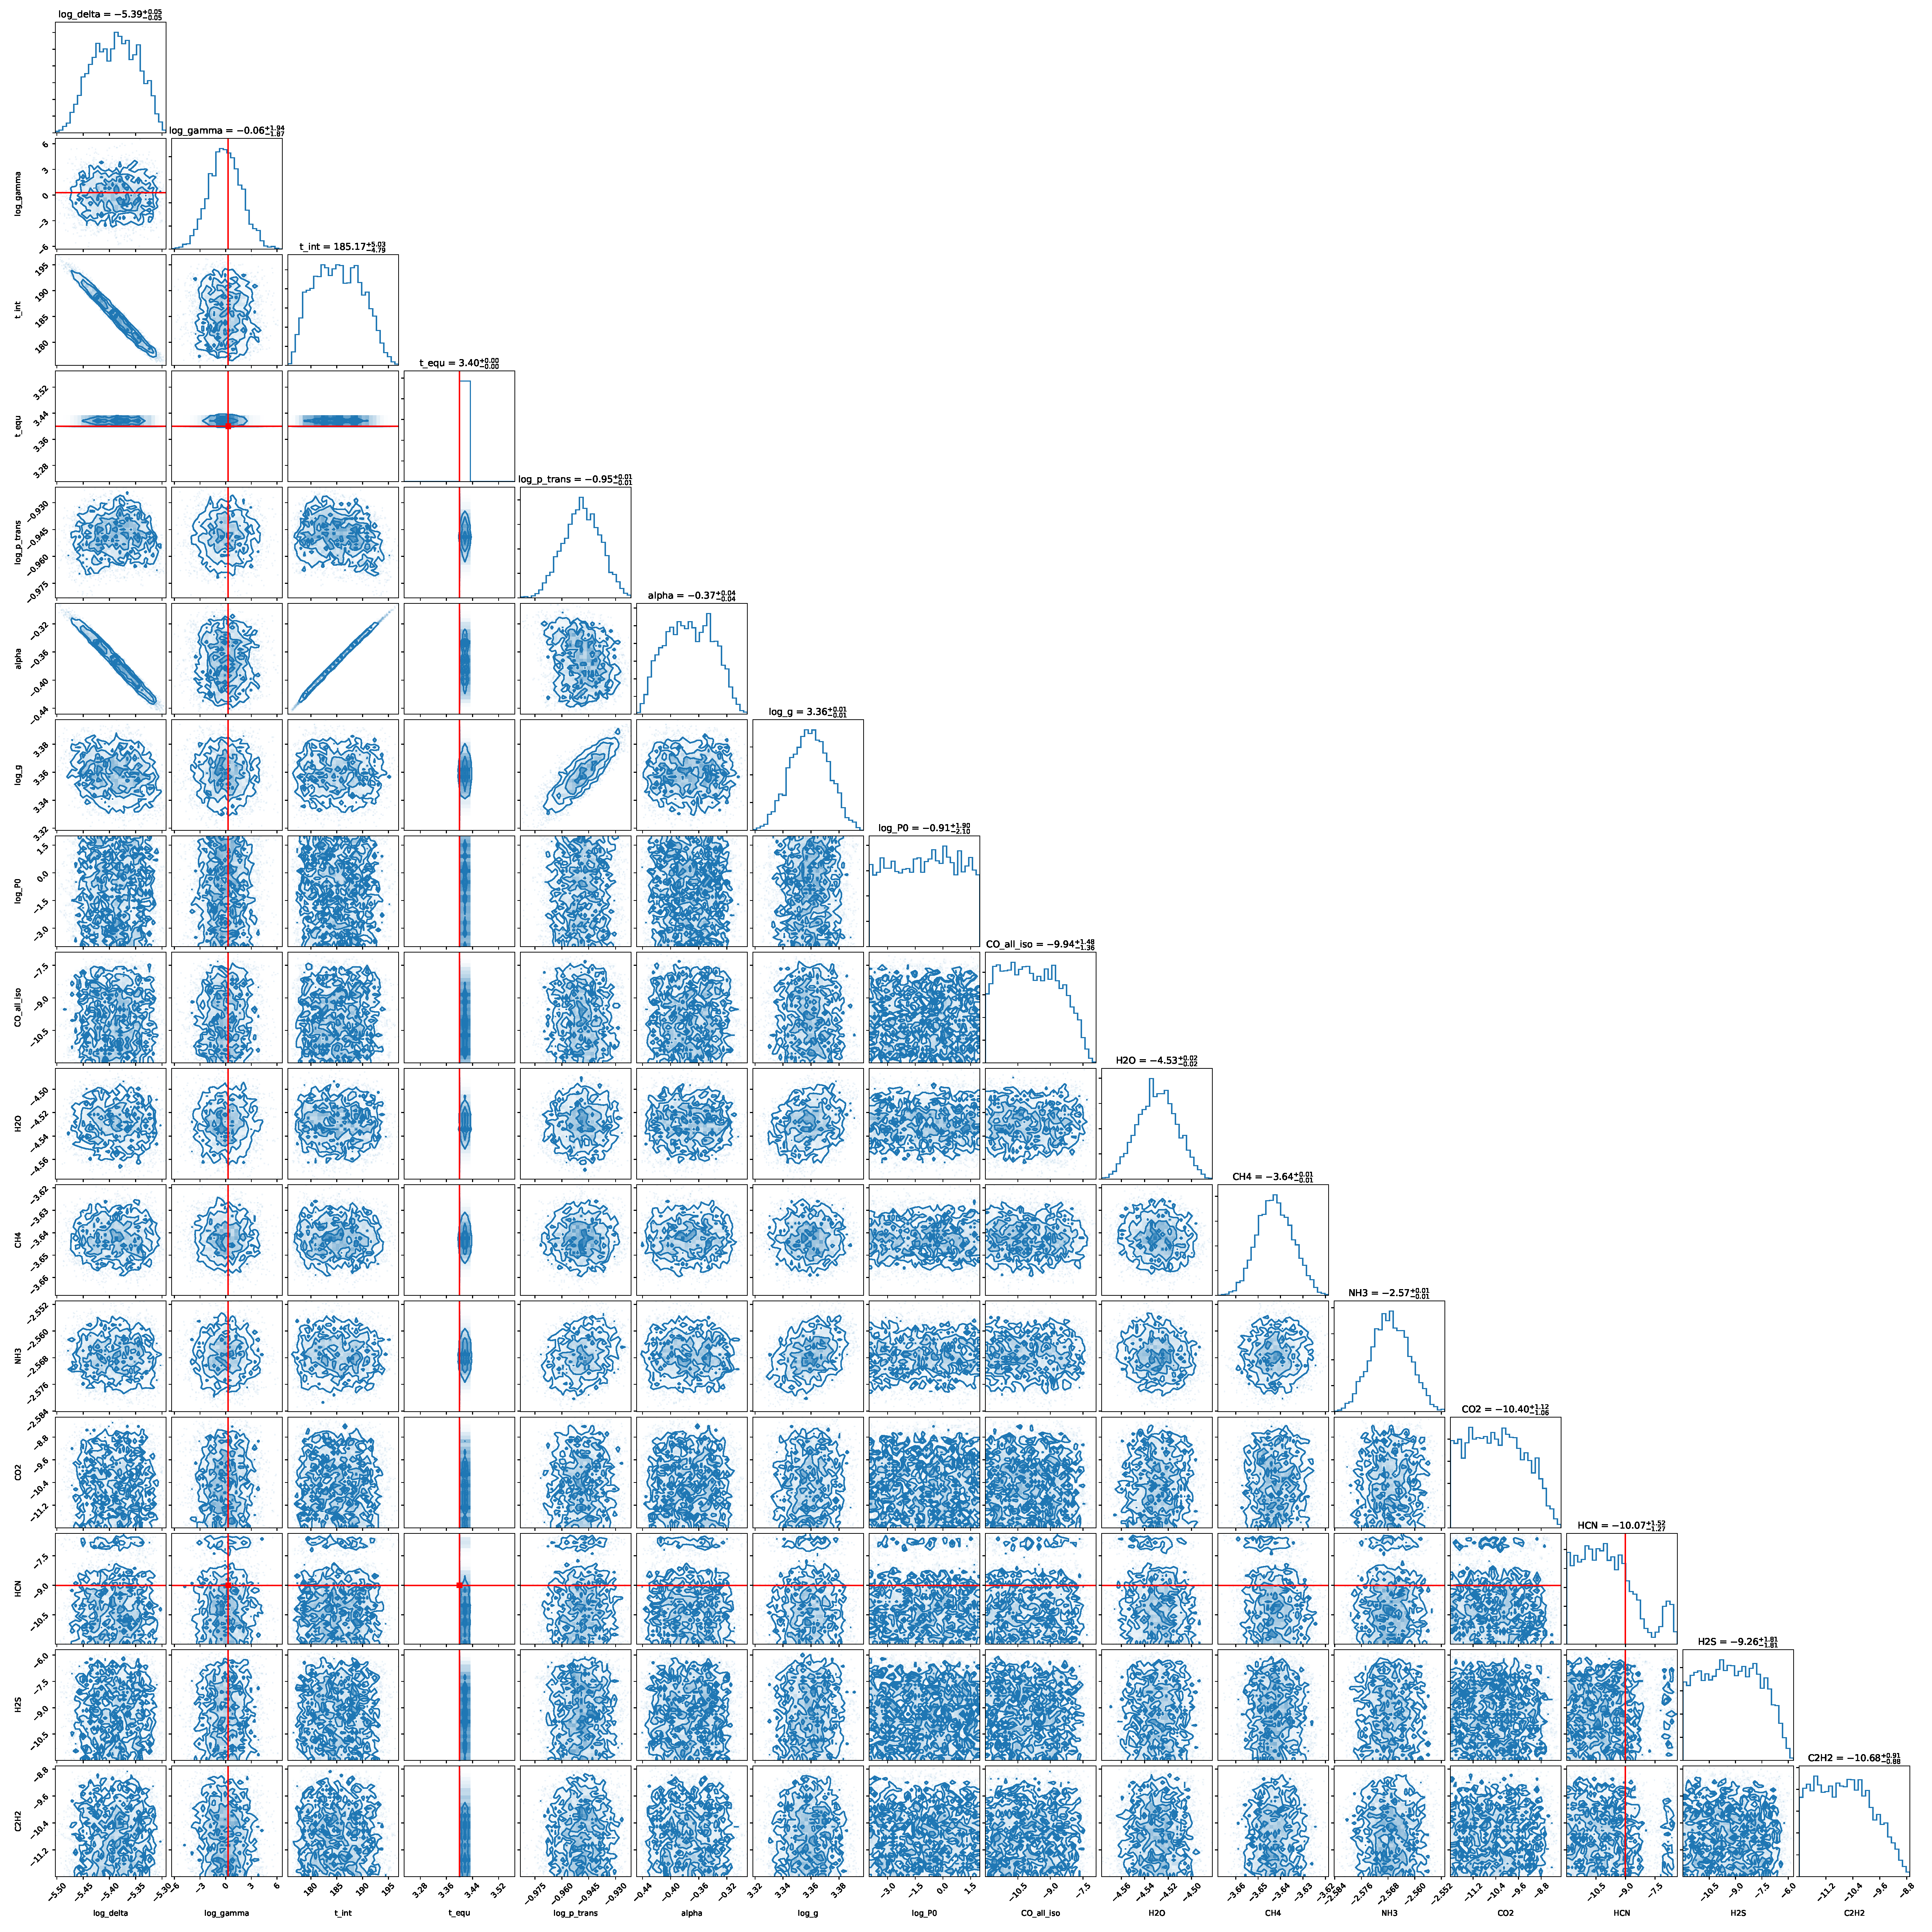
\includegraphics[width=\linewidth]{2M1207B_v2_fringing_corner}
	\caption{Posterior Distributions for 2M1207b.}
	\label{fig:post2M}
\end{figure}
\begin{figure}[h]
	%\includegraphics[content...]{imagefile}
	\caption{Pressure Temperature profile for}
	\label{fig:pres2M}
\end{figure}
\begin{figure}[h]
	%\includegraphics[content...]{imagefile}
	\caption{Best fit model for}
	\label{fig:bestfit2M}
\end{figure}

\subsection{WISE 0855}
\begin{figure}[h]
	%\includegraphics[content...]{imagefile}
	\caption{Posterior Distributions for}
	\label{fig:postWISE}
\end{figure}
\begin{figure}[h]
	\includegraphics[width=\linewidth]{WISE0855_ptsrc_onax_pt_env}
	\caption{Pressure Temperature profile for WISE 0855.}
	\label{fig:presWISE}
\end{figure}
\begin{figure}[h]
	\includegraphics[width=\linewidth]{BestfitBrownDwarf_fringe}
	\includegraphics[width=\linewidth]{BestfitWISE0855}
	\caption{Best fit model for WISE0855}
	\label{fig:bestfitWISE}
\end{figure}
\subsection{Discussion}
% This all ignores inherent issues that may be present in petitRADTRANS. However, the purpose of this work is not to realistically model atmospheres, but rather to show the extent to which current tools can retrieve input parameters. Other works such as \parencite{Barstow2020} have compared various retrieval and modelling tools, finding that while generally similar results are obtained, there are scenarios where different tools lead to different posterior distributions. 
	\chapter{Discussion and Conclusions}
\section{Summary of Results}
\subsection{Effects of fringing on cross correlations}
\subsection{Effects of fringing on atmospheric retrievals}
\subsection{Atmospheric retrievals with the MIRI MRS}
\section{Discussion}
\subsection{Implications for GTO Observations}
\subsection{Caveats and Limitations}
MIRISIM issues
JWST pipeline issues
petitRadTrans as input and output - validate models
petitRadTrans spectral resolution
1D models - planets aren't 1D \parencite{Taylor2020}
No background
\subsection{Future work}
Properly implement fringe model and correction
Clouds + variability
Designing better observing strategies
Comparing different spectral models
Extracting planet spectrum in contrast limited regime
\section{Conclusions}
	\appendix
\chapter{Appendix}
\section{Cross Correlations}
\begin{figure}[h]
	\includegraphics[width=\linewidth,trim=4cm 3.5cm 4cm 4.5cm, clip]{WISECrossCorTemplate}
	\caption{Cross correlation between the input template and the extracted spectra for WISE0855.}
\end{figure}
\begin{figure}[h]
	\includegraphics[width=\linewidth,trim=4cm 3.5cm 4cm 4.5cm, clip]{WISECO}
	\caption{Single species cross correlation between CO and WISE0855. The lack of significant spectral coverage results in a false positive detection.}
	\label{fig:wiseco}
\end{figure}
\begin{figure}[h]
	\includegraphics[width=\linewidth,trim=4cm 3.5cm 4cm 4.5cm, clip]{2M1207bCrossCorTemplate}
	\caption{Cross correlation between the input template and the extracted spectra for 2M1207b.}
\end{figure}
\begin{figure}[h]
	\includegraphics[width=\linewidth,trim=4cm 3.5cm 4cm 4.5cm, clip]{VHSCrossCorTemplateUncorrOnAxCH1}
	\caption{Cross correlation between the input template and the extracted spectra for VHS1256b. In this plot, the on axis point source has not been corrected with the extended source fringe flat, resulting in a higher SNR than with the correction.}
\end{figure}

\clearpage
\section{Package Requirements}
\verbatiminput{Chapters/requirements.txt}

	\clearpage
	% !TEX TS-program = pdflatex
% !TEX root = ../ArsClassica.tex

%*******************************************************
% Bibliography
%*******************************************************

%\bibliographystyle{ieeetr}
%\bibliography{thesis_bib}
%\nocite{*}
\printbibliography
\end{document}
